%%
%% Monte Carlo Pinpoint: Stochastic Coordinate Localization via VLM Probing
%% ACM sigconf format (CHI / UIST)
%%

\documentclass[sigconf,nonacm]{acmart}
%% Remove 'nonacm' when submitting to an actual ACM venue.

\usepackage{amsmath}
\let\Bbbk\relax
\usepackage{amssymb}
\usepackage{booktabs}
\usepackage{algorithm}
\usepackage{algpseudocode}
\usepackage{tikz}
\usetikzlibrary{positioning}
\usepackage{pgfplots}
\pgfplotsset{compat=1.18}
\usepackage{subcaption}
\usepackage{xcolor}
\usepackage{listings}

%% Listing style for pseudocode
\lstset{
  basicstyle=\ttfamily\small,
  keywordstyle=\color{blue},
  commentstyle=\color{gray},
  breaklines=true,
  frame=single
}

%% ----------------------------------------------------------------
%%  Metadata
%% ----------------------------------------------------------------
\title{Monte Carlo Pinpoint: Stochastic Coordinate Localization via VLM Probing}

\author{Tomio Hisanari}
\affiliation{%
  \institution{Independent Researcher}
  \country{Japan}
}
\email{tabby\_tomo\_srv@hotmail.co.jp}

%% ----------------------------------------------------------------
%%  Abstract
%% ----------------------------------------------------------------
\begin{abstract}
For AI agents that autonomously operate graphical user interfaces,
accurate coordinate localization on screen remains a fundamental challenge.
The dominant approach, Set-of-Mark (SoM) prompting, relies on
OpenCV contour detection and can only mark \emph{UI elements}.
However, real-world tasks often require localizing arbitrary semantic
positions---the tip of a character's nose, a specific object inside a painting,
a defect on a textured surface---that are \emph{not} UI elements at all.

We propose \textbf{Monte Carlo Pinpoint}, a three-phase method that
converts coordinate estimation (a regression problem) into a ranking
problem by asking a Vision--Language Model (VLM)
``\emph{Which dot is closest to the target?}''
Phase~1 uses deterministic grid bisection to narrow the search to a
coarse region ($\pm G$ pixels).
Phase~1.5 elicits an \emph{anchor declaration} from the VLM to stabilize
subsequent judgments.
Phase~2 places a deterministic seven-point hexagonal stencil inside
the region, asks the VLM to select the closest dot with majority vote,
and halves the search radius on each majority-HIT round (with bounded
MISS retries that do not shrink the radius)---guaranteeing convergence
when the target lies within the initial search disk and the VLM
selects the closest dot on each HIT round.

We prove that the expected number of VLM queries is
$O(v \cdot \log(s_0/\varepsilon))$, where $v$ is the majority vote
size, $s_0$ the initial search radius, and $\varepsilon$ the target
precision---a logarithmic improvement over the $O(s_0^2)$ cost of
exhaustive search.
On a benchmark of 50 synthetic conditions across five categories,
evaluated with a single VLM backbone and one trial per condition,
Pinpoint---among the empirically evaluated Grid baseline and Pinpoint
variants---is the only method in this evaluated set that achieves
practical accuracy on the non-UI targets in this synthetic benchmark,
while remaining competitive on standard UI elements; broader
evaluation across additional VLM backbones, real-desktop tasks,
repeat trials, and additional baselines (e.g., Direct/SoM-family
methods) is reserved for future work
(\S\ref{sec:limitations}).
We additionally distill a failure-mode taxonomy of VLM
coordinate-localization hallucinations (the H-$\ast$ family of
seven cognitive failure classes) and benchmark-execution
operational failures (the O-$\ast$ family covering pipeline,
rate-limit, credit-exhaustion, and audit-trail layers), with
corresponding guardrail countermeasures grounded in real
benchmark-execution incidents.
\end{abstract}

%% ----------------------------------------------------------------
%%  CCS Concepts and Keywords
%% ----------------------------------------------------------------
\begin{CCSXML}
<ccs2012>
   <concept>
       <concept_id>10003120.10003121.10003122</concept_id>
       <concept_desc>Human-centered computing~HCI design and evaluation methods</concept_desc>
       <concept_significance>500</concept_significance>
   </concept>
   <concept>
       <concept_id>10010147.10010178</concept_id>
       <concept_desc>Computing methodologies~Artificial intelligence</concept_desc>
       <concept_significance>500</concept_significance>
   </concept>
</ccs2012>
\end{CCSXML}

\ccsdesc[500]{Human-centered computing~HCI design and evaluation methods}
\ccsdesc[500]{Computing methodologies~Artificial intelligence}

\keywords{GUI agents, coordinate localization, vision--language models,
  Monte Carlo methods, visual prompting}

%% ----------------------------------------------------------------
\begin{document}
\maketitle

%% Allow modest extra inter-word stretch on otherwise unfixable lines
%% (e.g., paragraphs containing long monospace identifiers and
%% multi-key citations).  Avoids visual overflow without altering text.
%% Bumped 3em -> 5em in Bundle 2.17 M4 to clear ~48pt overfull on
%% lines containing long monospace VLM identifiers.
\setlength{\emergencystretch}{5em}
%% Permit hyperref-managed boxes (cite, ref, url) to break across lines.
\hypersetup{breaklinks=true}

%% ================================================================
%%  1. INTRODUCTION
%% ================================================================
\section{Introduction}

\subsection{Problem Statement}

GUI agents such as CogAgent, SeeClick, and Claude Computer Use possess
the ability to ``see the screen and take actions,'' yet the
\emph{accuracy of coordinate localization} remains their principal
bottleneck~\cite{seeclick,uitars}.
When a VLM is asked directly for the coordinates of an on-screen
element, it frequently \emph{hallucinates}---producing estimates that
are tens to hundreds of pixels away from the true
location~\cite{localization-biases}.
The very existence of dedicated Computer Use APIs is evidence that
VLM-based coordinate regression cannot yet be trusted.

\subsection{Limitations of Existing Approaches}

\begin{table}[t]
\caption{Limitations of existing coordinate localization approaches.}
\label{tab:existing-limits}
\resizebox{\columnwidth}{!}{%
\begin{tabular}{lll}
\toprule
\textbf{Method} & \textbf{Principle} & \textbf{Limitation} \\
\midrule
Direct regression & Ask VLM for coords & Hallucination ($\pm$50--200\,px) \\
SoM & OpenCV contours + labels & UI elements only \\
UI Automation & OS accessibility API & Programmable elements only \\
Template matching & Pre-registered images & Requires prior registration \\
\bottomrule
\end{tabular}%
}
\end{table}

Table~\ref{tab:existing-limits} summarizes the landscape.  The
\textbf{core gap} is that no existing method can localize an
\emph{arbitrary semantic position inside an image} to pixel precision.

\subsection{Contributions}

This paper makes five contributions:

\begin{enumerate}
  \item \textbf{Monte Carlo Pinpoint algorithm}: a three-layer
    architecture combining deterministic grid bisection, anchor
    declaration, and deterministic hex-stencil probing with HIT-only
    radius halving.
  \item \textbf{Theoretical analysis}: derivation of the expected
    query count $O(v \cdot \log(s_0/\varepsilon))$ via closest-dot
    convergence, including a model of VLM judgment error impact.
  \item \textbf{Benchmark}: empirical evaluation across five categories
    (UI buttons, dense UI, natural images, ambiguous targets,
    precision tests) with 50~conditions.
  \item \textbf{Open-source implementation}: released as the
    \texttt{pinpoint} tool in the \texttt{video2ai-desktop} MCP server
    (entry point: \texttt{mcp\_server.py} at the repository root).
    The Phase~2 dot-placement primitive (\texttt{pinpoint\_core.py})
    is shared with the benchmark harness, preventing future
    dot-placement drift between the two paths.  Reported hex-stencil
    numerical results are reproduced from the 50-case rerun on the
    CLI subscription variant (Table~\ref{tab:hex-stencil-50case}).
  \item \textbf{Failure mode analysis}: a taxonomy of VLM
    coordinate-localization cognitive failures (the H-$\ast$
    taxonomy of seven classes) and benchmark-execution
    operational failures (the O-$\ast$ family covering pipeline,
    rate-limit, credit-exhaustion, and audit-trail layers), with
    matching pipeline-layer and audit-emission countermeasures
    grounded in a series of real benchmark-execution incidents
    and engineering experience.
\end{enumerate}


%% ================================================================
%%  2. RELATED WORK
%% ================================================================
\section{Related Work}
\label{sec:related-work}

\subsection{Direct Coordinate Regression}

Several systems ask VLMs to output coordinates as text tokens.
SeeClick~\cite{seeclick} fine-tunes a VLM specifically for GUI
grounding and proposes the ScreenSpot benchmark.
UI-TARS~\cite{uitars} operates from screenshots alone with a
coordinate-based action space.
OS-ATLAS~\cite{osatlas} compiles a 13\,M-sample grounding dataset
and finds 11.3\% mislabeled entries in ScreenSpot.
Recent work~\cite{localization-biases} demonstrates systematic spatial
biases in VLM coordinate predictions, providing theoretical
justification for Pinpoint's regression-to-classification transform.
Explicit position-to-coordinate mapping~\cite{pos2coord} analyzes the
limits of generating coordinates as text tokens and improves regression
through explicit position encoding; Pinpoint instead abandons
regression entirely.
Talking Points~\cite{rusanovsky2025talkingpoints} pairs a point
descriptor with a learned localizer for pixel-level grounding from
natural-language descriptions; Pinpoint differs in remaining training-
free and in deriving its precision from a Monte~Carlo voting budget
rather than from a regressed coordinate.

\subsection{Fine-tuned Grounding Models}

UGround~\cite{uground} trains a universal GUI grounding model on
large-scale synthetic web data.
Aria-UI~\cite{ariaui} achieves purely visual grounding without HTML or
accessibility trees but depends on task-specific training.
ShowUI~\cite{showui} introduces UI-guided token selection for
efficient screenshot processing.
MolmoPoint~\cite{molmopoint} adds grounding-specific tokens to the VLM
architecture.
Pinpoint requires \emph{no fine-tuning} and works with any off-the-shelf VLM.

\subsection{Segmentation-Dependent Methods (SoM Family)}

Set-of-Mark (SoM)~\cite{som} overlays numbered labels on regions
detected by segmentation (SAM / OpenCV) and asks the VLM to select
among them.  It is the closest prior work to Pinpoint but is
\emph{inherently limited to segmentable regions}---i.e., UI elements.
OmniParser~\cite{omniparser} uses fine-tuned detection and captioning
models, again limited to UI elements.
MEGA-GUI~\cite{megagui} adopts a coarse ROI selection followed by
fine localization, but relies on trained models.
Pinpoint replaces segmentation with a deterministic hex-stencil dot
arrangement, eliminating the dependency on element detectors.

\subsection{Zoom and Iterative Refinement}

This family of methods is conceptually closest to Pinpoint's Phase~1.
RegionFocus~\cite{regionfocus} zooms into candidate regions at test
time and re-queries the VLM---training-free but lacking a
probabilistic refinement phase.
AdaZoom-GUI~\cite{adazoom} adapts zoom level to element size and
refines instructions at each step, resembling Phase~1 + Phase~1.5
but without Monte Carlo refinement.
A systematic study of zooming~\cite{zooming-study} confirms that zoom
improves GUI grounding accuracy but does not address how to go beyond
the zoom limit.
GUI-Spotlight~\cite{gui-spotlight} uses iterative spotlighting with
think-with-image, requiring training.
Chain-of-Ground~\cite{chain-of-ground} narrows the search space
through iterative reasoning steps in text; Pinpoint uses \emph{visual}
overlays (grids, dots) as the reasoning medium.
Several contemporaneous works extend the zoom paradigm with explicit
uncertainty signals: UI-Zoomer~\cite{tang2026uizoomer} drives zoom
selection by token-distribution uncertainty,
AutoFocus~\cite{yao2026autofocus} uses token-level perplexity to
model spatial uncertainty for active visual search, Zoom
Consistency~\cite{kim2026zoomconsistency} shows that geometric
agreement across zoom steps is itself a calibration-free confidence
signal, and BAMI~\cite{zhang2026bami} addresses precision and
ambiguity biases in {GUI} grounding through training-free coarse-to-
fine focusing with candidate selection; Pinpoint instead uses
deterministic grid bisection followed by Monte Carlo voting, deriving
its certainty guarantee from a sample budget rather than from a
learned uncertainty estimator or a focusing heuristic.

\subsection{Test-Time Voting and Scaling}

GUI-RC~\cite{guirc} constructs a spatial voting grid from multiple
predictions and uses region consistency---the most directly related
work.  However, GUI-RC aggregates predictions \emph{across queries},
whereas Pinpoint converts the problem to classification \emph{within a
single query}.
DiMo-GUI~\cite{dimogui} provides a training-free framework with
dynamic visual grounding and modality switching.
GTA1~\cite{gta1} learns test-time scaling via RL; Pinpoint is purely
inference-time.
GAIA~\cite{gaia} uses best-of-$N$ selection, conceptually similar to
Pinpoint's majority vote but over complete action predictions rather
than dot classifications.

\subsection{Coordinate-Free Approaches}

GUI-Actor~\cite{guiactor} replaces coordinate regression with an
attention-based action head.  While it shares Pinpoint's problem
recognition (coordinate regression is ill-suited for VLMs), it
requires \emph{architectural changes}; Pinpoint is a pure prompting
strategy applicable to any VLM.

\subsection{Visual Prompting}

VP-VLA~\cite{vpvla} overlays spatial anchors (crosshairs, bounding
boxes) on visual input for robotics tasks, sharing Pinpoint's
philosophy of augmenting images with visual prompts.
V2P~\cite{v2p} uses background suppression and center peaking to
improve coordinate regression---still a regression approach addressed
via data augmentation, whereas Pinpoint replaces regression with
classification.

\subsection{Agent Orchestration and Harnesses}

Concurrent with this work, a wave of open-source orchestration
specs and harness patterns has emerged at the systems level:
OpenAI's Symphony~\cite{openai2026symphony,openai2026symphonyrepo},
released 2026-04-27 under Apache~2.0, treats a Linear
project board as the control plane for autonomous Codex
agents, with workflow loaders, retry backoff, and structured
logging surfaces; alongside this, industry harnesses such
as Anthropic's three-agent pattern~\cite{anthropic2026threeagentharness}
decompose long-running tasks across planner / generator /
evaluator phases (analysed further in
Section~\ref{sec:discussion-stage-c}).  Symphony's scope is full
task lifecycle orchestration---issue pickup, agent restart,
PR landing---operating at the workflow-orchestration layer,
above the per-task agent layer that hosts primitives like
Pinpoint.  Pinpoint, by contrast, uses agentic tool-use as
a \emph{probing primitive}: a single coordinate query is
wrapped in a structured tool call (Section~\ref{sec:results},
the CLI subscription variant), and $N\!=\!3$ plurality voting
on tool-use responses (the CLI plurality-vote variant) yields
measurable selectivity gains
(Section~\ref{sec:aggregation-discussion}).  The two layers
compose: a Symphony-style orchestrator could dispatch
Pinpoint as a coordinate-finding tool.  We position Pinpoint
as the lower-level visual-grounding component such an
orchestration stack would invoke.

Concurrent work by Augment Code introduces
``Intent''~\cite{augmentcode2026intent}, an agentic development
environment that ``coordinates agents through a shared living
spec rather than wiring them together through code''.  Intent
employs a Coordinator--Implementor--Verifier topology---a
Coordinator agent proposes a plan as a spec, Implementor agents
execute in parallel waves, and a Verifier checks results against
the spec---and thus shares the three-role harness structure
under which Pinpoint was developed.  Two axes distinguish the
present work from such spec-driven orchestrators: a
heterogeneous-model consultant tier that supplies independent
cross-validation of same-model reviewer agreement (Codex CLI in
our deployment), and a visual--plus--text dual-surface
programming model that neither pure-CLI orchestrators (e.g.,
Symphony or Intent) nor pure-visual workflow platforms occupy.

\subsection{System-layer Computer Use and GUI Grounding}

Beyond the algorithmic sub-pixel grounding primitives we
survey above, a complementary research line addresses
the \emph{system layer}: how an agent should perceive,
navigate, and click within full desktop and browser
environments.  OpenAI's Computer-Using
Agent~\cite{openai2025cua} reports OSWorld 38.1\,\%,
WebArena 58.1\,\%, and WebVoyager 87.0\,\%
(self-reported, January 2025).  Anthropic's
computer-use tool~\cite{anthropic2026computeruse}
provides 1\,:\,1 native coordinate handling for
screenshots up to 2576\,px on the long edge with an
explicit \texttt{zoom} action for inspecting
sub-regions at full resolution.  On the
high-resolution professional grounding benchmark
ScreenSpot-Pro~\cite{li2025screenspotpro}, accuracy
has progressed from an initial 18.9\,\% to
ScreenSeekeR's 48.1\,\% via cascaded visual search,
GUI-Actor-7B + Qwen2.5-VL-7B's 44.6\,\% via
coordinate-free attention~\cite{guiactor},
OSWorld-G/Jedi-7B's 39.5\,\% via grounding-data
scaling~\cite{xie2025jedi}, and RegionFocus's
61.6\,\% via test-time zoom on a Qwen2.5-VL-72B
base~\cite{regionfocus}.  The published values remain
below human level for the highest-resolution
targets, and apples-to-apples comparison is
complicated by base-model size and search-augmentation
variation.  Pinpoint, the algorithm-layer primitive
we present, is positioned to plug into any of these
system-layer harnesses as a deterministic
coordinate-inference fallback for boundary-ambiguous
and sub-pixel targets that remain difficult for
end-to-end VLMs.

\subsection{Agent Failure Taxonomies and Incident Analysis}
\label{sec:agent-failure-taxonomies}

Beyond the algorithm-layer and system-layer prior art surveyed
above, a parallel literature classifies the failures of
\emph{agent systems themselves}.  We position our
H-$\ast$/O-$\ast$ split against five lines of this work.
Recent multi-agent-system work classifies traces into
system-design, inter-agent-misalignment, and task-verification
failures~\cite{cemri2025mast}; our taxonomy instead separates
VLM-internal visual grounding hallucinations from operational
failures in the surrounding benchmark and agent infrastructure.
At the single-agent level, AgentErrorTaxonomy localizes
failures across memory, reflection, planning, action, and
system-level modules~\cite{zhu2025agenterror}, whereas our
H/O split isolates visual-grounding hallucinations from
non-model operational faults in the benchmark harness.
On the software-engineering side, empirical studies of
agentic-AI repositories classify faults by type, symptom,
root cause, and architectural
dimension~\cite{shah2026agenticfaults}; our O-$\ast$ family
narrows that lens to the operational layers that affected a
VLM grounding benchmark.
Agent-incident-analysis frameworks distinguish system-related,
contextual, and cognitive
factors~\cite{ezell2025incidentanalysis}; our taxonomy
operationalizes a related split at benchmark scale by
separating VLM coordinate-localization hallucinations from
pipeline, rate-limit, credit-exhaustion, and audit-trail
failures.
Two transferred-discipline analogues motivate the layered
diagnostic stance: HFACS~\cite{wiegmann2003hfacs} separates
immediate unsafe acts from latent organizational conditions,
a stance our O-$\ast$ stack applies to benchmark-execution
workflows; and ODC~\cite{chillarege1992odc} treats defect
classifications as in-process measurement signals, mirroring
how separating H-$\ast$ and O-$\ast$ preserves whether
accuracy loss came from model grounding or operational
infrastructure.
None of the above provides the specific
cognitive-vs-operational separation we propose for VLM
grounding systems, but each informs where our taxonomy sits
in the broader agent-failure analysis landscape.

\subsection{Positioning of This Work}

\begin{table}[t]
\caption{Comparison of approaches. Pinpoint combines deterministic
  grid narrowing, anchor declaration, and hex-stencil dot voting---a
  combination absent from all prior work.}
\label{tab:positioning}
\resizebox{\columnwidth}{!}{%
\begin{tabular}{lll}
\toprule
\textbf{Approach} & \textbf{Representative} & \textbf{Pinpoint Advantage} \\
\midrule
Direct regression & SeeClick, UI-TARS & Avoids hallucination via classification \\
Fine-tuning & UGround, Aria-UI & Training-free; any VLM \\
Segmentation-dep. & SoM, OmniParser & No detector; non-UI targets \\
Zoom refinement & RegionFocus & Probabilistic phase beyond zoom limit \\
Test-time voting & GUI-RC, GAIA & Intra-query classification voting \\
Architecture change & GUI-Actor & Prompting only; no model changes \\
\bottomrule
\end{tabular}%
}
\end{table}

Table~\ref{tab:positioning} summarizes the positioning.
No existing method combines all three phases of Pinpoint:
deterministic grid narrowing, anchor-based self-consistency, and
hex-stencil dot voting.
The use of distinctly colored hex-stencil dots for \emph{intra-query
regression-to-classification} conversion is novel.


%% ================================================================
%%  3. METHOD
%% ================================================================
\section{Method}

\subsection{Problem Formalization}
\label{sec:formalization}

\textbf{Input:} An image $I$ and a natural-language target description
$T$ (e.g., ``the center of the gear icon'').

\textbf{Output:} Target coordinates $(x^*, y^*) \pm \varepsilon$ pixels.

\textbf{Oracle:} A VLM $V(I', Q) \to A$, which returns an answer $A$
to a textual question $Q$ given a (possibly annotated) image $I'$.

\textbf{Core transformation:} We convert coordinate estimation
(regression) into the ranking question ``\emph{Which dot is closest
to the target?}''

\subsection{Algorithm Overview}
\label{sec:overview}

The algorithm proceeds in three (optionally four) phases:

\begin{description}
  \item[Phase 1 --- Deterministic Grid Search.]
    Narrows the target to a $\pm G$-pixel region via axis-independent
    binary search over grid cells.
  \item[Phase 1.5 --- Anchor Declaration (Guardrail).]
    Elicits a precise natural-language self-declaration from the VLM
    of \emph{exactly which pixel} it aims at, anchoring subsequent
    judgments.
  \item[Phase 2 --- Hex-Stencil Dot Probing.]
    Places a deterministic seven-point hexagonal stencil ($k{=}7$) in
    the region, asks the VLM which dot is closest to the anchor, and
    halves the search radius on each majority-HIT round (with bounded
    MISS retries that do not shrink the radius); converges under the
    containment and judgment assumptions stated in
    Section~\ref{sec:convergence}.
  \item[Phase 3 --- Super-Zoom Refinement (Optional).]
    For $\varepsilon < 5$, re-probes at extreme magnification around the
    Phase~2 hit point to reach 1\,px accuracy.
\end{description}

Figure~\ref{fig:overview} illustrates the flow.

\begin{figure}[t]
  \centering
  \resizebox{\columnwidth}{!}{%% algorithm_overview.tex — Phase 1 → 1.5 → 2 → 3 flow diagram
%% Include via %% algorithm_overview.tex — Phase 1 → 1.5 → 2 → 3 flow diagram
%% Include via %% algorithm_overview.tex — Phase 1 → 1.5 → 2 → 3 flow diagram
%% Include via \input{figures/algorithm_overview} in main.tex

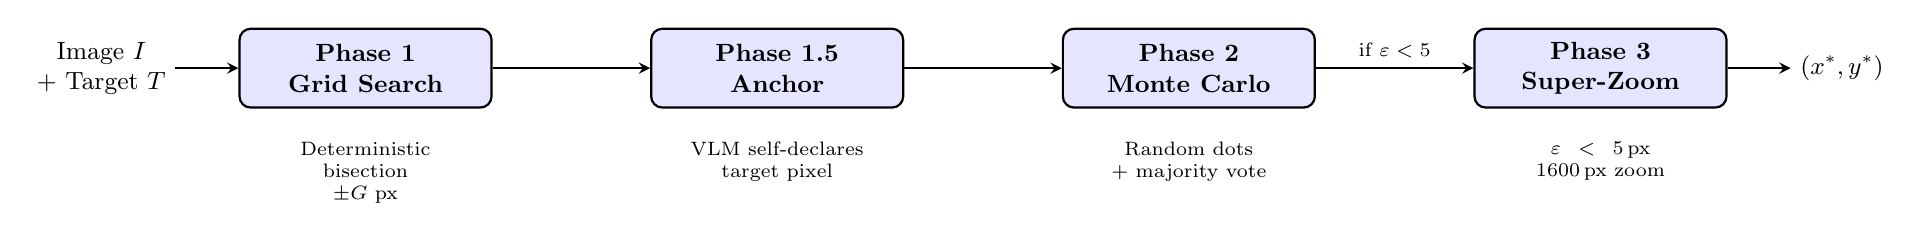
\begin{tikzpicture}[
    node distance=1.8cm,
    phase/.style={
      rectangle, rounded corners=4pt, draw=black, thick,
      fill=blue!10, minimum width=3.2cm, minimum height=1cm,
      align=center, font=\small\bfseries
    },
    detail/.style={
      font=\scriptsize, align=center, text width=3.2cm
    },
    arrow/.style={->, thick, >=stealth},
  ]

  %% Nodes
  \node[phase] (p1) {Phase 1\\Grid Search};
  \node[phase, right=2.0cm of p1] (p15) {Phase 1.5\\Anchor};
  \node[phase, right=2.0cm of p15] (p2) {Phase 2\\Monte Carlo};
  \node[phase, right=2.0cm of p2] (p3) {Phase 3\\Super-Zoom};

  %% Detail labels below
  \node[detail, below=0.3cm of p1]
    {Deterministic\\bisection\\$\pm G$ px};
  \node[detail, below=0.3cm of p15]
    {VLM self-declares\\target pixel};
  \node[detail, below=0.3cm of p2]
    {Random dots\\+ majority vote};
  \node[detail, below=0.3cm of p3]
    {$\varepsilon < 5$\,px\\1600\,px zoom};

  %% Arrows
  \draw[arrow] (p1) -- (p15);
  \draw[arrow] (p15) -- (p2);
  \draw[arrow] (p2) -- node[above, font=\scriptsize] {if $\varepsilon<5$} (p3);

  %% Input / Output
  \node[left=0.8cm of p1, font=\small, align=center] (input)
    {Image $I$\\+ Target $T$};
  \node[right=0.8cm of p3, font=\small] (output) {$(x^*, y^*)$};
  \draw[arrow] (input) -- (p1);
  \draw[arrow] (p3) -- (output);

\end{tikzpicture}
 in main.tex

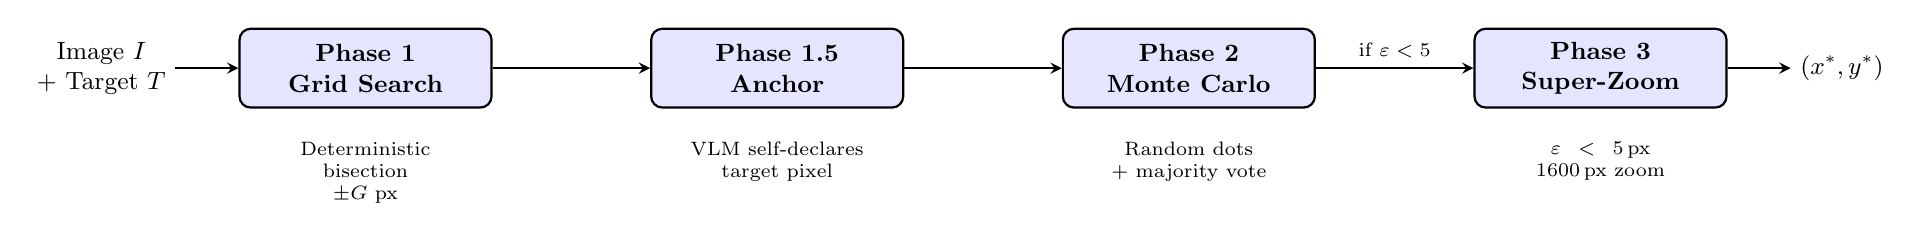
\begin{tikzpicture}[
    node distance=1.8cm,
    phase/.style={
      rectangle, rounded corners=4pt, draw=black, thick,
      fill=blue!10, minimum width=3.2cm, minimum height=1cm,
      align=center, font=\small\bfseries
    },
    detail/.style={
      font=\scriptsize, align=center, text width=3.2cm
    },
    arrow/.style={->, thick, >=stealth},
  ]

  %% Nodes
  \node[phase] (p1) {Phase 1\\Grid Search};
  \node[phase, right=2.0cm of p1] (p15) {Phase 1.5\\Anchor};
  \node[phase, right=2.0cm of p15] (p2) {Phase 2\\Monte Carlo};
  \node[phase, right=2.0cm of p2] (p3) {Phase 3\\Super-Zoom};

  %% Detail labels below
  \node[detail, below=0.3cm of p1]
    {Deterministic\\bisection\\$\pm G$ px};
  \node[detail, below=0.3cm of p15]
    {VLM self-declares\\target pixel};
  \node[detail, below=0.3cm of p2]
    {Random dots\\+ majority vote};
  \node[detail, below=0.3cm of p3]
    {$\varepsilon < 5$\,px\\1600\,px zoom};

  %% Arrows
  \draw[arrow] (p1) -- (p15);
  \draw[arrow] (p15) -- (p2);
  \draw[arrow] (p2) -- node[above, font=\scriptsize] {if $\varepsilon<5$} (p3);

  %% Input / Output
  \node[left=0.8cm of p1, font=\small, align=center] (input)
    {Image $I$\\+ Target $T$};
  \node[right=0.8cm of p3, font=\small] (output) {$(x^*, y^*)$};
  \draw[arrow] (input) -- (p1);
  \draw[arrow] (p3) -- (output);

\end{tikzpicture}
 in main.tex

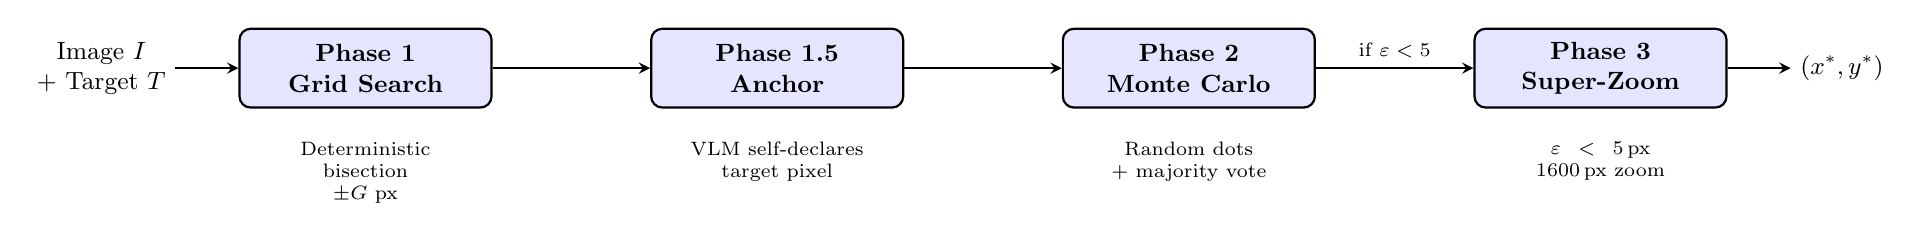
\begin{tikzpicture}[
    node distance=1.8cm,
    phase/.style={
      rectangle, rounded corners=4pt, draw=black, thick,
      fill=blue!10, minimum width=3.2cm, minimum height=1cm,
      align=center, font=\small\bfseries
    },
    detail/.style={
      font=\scriptsize, align=center, text width=3.2cm
    },
    arrow/.style={->, thick, >=stealth},
  ]

  %% Nodes
  \node[phase] (p1) {Phase 1\\Grid Search};
  \node[phase, right=2.0cm of p1] (p15) {Phase 1.5\\Anchor};
  \node[phase, right=2.0cm of p15] (p2) {Phase 2\\Monte Carlo};
  \node[phase, right=2.0cm of p2] (p3) {Phase 3\\Super-Zoom};

  %% Detail labels below
  \node[detail, below=0.3cm of p1]
    {Deterministic\\bisection\\$\pm G$ px};
  \node[detail, below=0.3cm of p15]
    {VLM self-declares\\target pixel};
  \node[detail, below=0.3cm of p2]
    {Random dots\\+ majority vote};
  \node[detail, below=0.3cm of p3]
    {$\varepsilon < 5$\,px\\1600\,px zoom};

  %% Arrows
  \draw[arrow] (p1) -- (p15);
  \draw[arrow] (p15) -- (p2);
  \draw[arrow] (p2) -- node[above, font=\scriptsize] {if $\varepsilon<5$} (p3);

  %% Input / Output
  \node[left=0.8cm of p1, font=\small, align=center] (input)
    {Image $I$\\+ Target $T$};
  \node[right=0.8cm of p3, font=\small] (output) {$(x^*, y^*)$};
  \draw[arrow] (input) -- (p1);
  \draw[arrow] (p3) -- (output);

\end{tikzpicture}
}
  \caption{Overview of the Monte Carlo Pinpoint pipeline.
    Phase~1 uses deterministic grid bisection; Phase~1.5 elicits an
    anchor declaration; Phase~2 applies deterministic hex-stencil
    probing with HIT-only radius halving and majority vote; Phase~3
    optionally refines to 1\,px precision.}
  \label{fig:overview}
  \Description{Block diagram of the four-phase Monte Carlo Pinpoint
    pipeline showing data flow from an input screenshot through
    Phase~1 deterministic grid bisection, Phase~1.5 anchor
    declaration, Phase~2 deterministic hex-stencil probing with
    majority voting and HIT-only radius halving, and an optional
    Phase~3 sub-pixel refinement step.}
\end{figure}


\subsection{Phase 1: Deterministic Grid Search}
\label{sec:phase1}

The $X$ and $Y$ axes are searched independently via binary bisection.
At each step, $n$ labeled grid lines are drawn on the image and the VLM
is asked ``\emph{Which line is closest to the target?}''  The VLM
replies with either an exact line (``L5'') or a between-lines interval
(``B3-4'').  Each response narrows the search region by a factor of
$\sim n$.

Two refinement mechanisms improve accuracy:

\begin{itemize}
  \item \textbf{Force zoom on first exact hit.}
    When the VLM reports an exact line on the first iteration, the
    result is treated as a between-lines interval spanning the adjacent
    lines (e.g., L5 $\to$ B4-6).  This forces a zoom refinement pass,
    mitigating VLM overconfidence at coarse scale.
  \item \textbf{Zoom mode.}
    When the search interval drops below $w/3$ pixels, the region is
    cropped and magnified to 1200\,px before re-querying.  This
    provides the VLM with higher-resolution input for the final
    bisection steps.  Image dimensions are clamped to 7900\,px to
    respect API limits.
\end{itemize}

\textbf{Failure fallback.}  If the grid search fails to locate the
target on either axis (VLM returns ``NONE''), the algorithm falls back
to a single direct VLM coordinate estimation query for the failed
axis.  This adds one query but prevents catastrophic failure where the
search center defaults to the image midpoint.

Each axis requires 2--4 VLM queries (typically 2 normal + 1--2 zoom).
Temperature is set to~0 for reproducibility.


\subsection{Phase 1.5: Anchor Declaration}
\label{sec:anchor}

Before entering the stochastic phase, we stabilize the VLM's judgment
criterion:

\begin{enumerate}
  \item The Phase~1 region is cropped and magnified.
  \item The VLM is asked to \emph{declare} in natural language
    the exact pixel it aims at---e.g., ``the gear icon'' becomes
    ``the exact center pixel of the gear icon's hub circle.''
  \item This declaration is used as the judgment criterion for all
    Phase~2 rounds.
  \item On the ABSENT wider-crop retry path, the anchor is
    re-requested; periodic re-declaration and semantic drift
    comparison are reserved as future / interactive-server
    guardrails.
\end{enumerate}

\textbf{Failure recovery.}  If the VLM cannot identify the target in
the initial crop (detected by responses beginning with ``I cannot
locate\ldots''), the crop is widened to $\pm w/3$ pixels (one-third
of the image dimension) and the anchor is re-requested.  This handles
cases where Phase~1's grid estimate is sufficiently inaccurate that the
target falls outside the narrow context crop.

\textbf{Rationale.} VLMs tend to \emph{drift} in their interpretation
of the target across multiple rounds.  An explicit anchor declaration
forces consistency and enables metacognitive correction when drift is
detected.


\subsection{Phase 2: Monte Carlo Dot Probing}
\label{sec:phase2}

Phase~2 uses a \emph{closest-dot convergence} strategy with a
deterministic seven-point hexagonal half-net rather than a binary
HIT/MISS test.  Each round proceeds as follows:

\begin{enumerate}
  \item Place the seven-point hexagonal stencil (one center dot,
    six on the ring of radius $\frac{\sqrt{3}}{2}\,s$ at $60^\circ$
    increments) inside the current search disk centered at
    $(\hat{x}, \hat{y})$ with radius $s$.
  \item Crop the context area ($3 \times s$) and magnify to a
    no-loss capped image (for Claude-class VLMs, 1024\,px on the
    longer axis).
  \item Annotate each dot with a numbered label and a unique color
    (adaptively selected for background contrast).
  \item Ask the VLM: ``\emph{Which dot is closest to the anchor
    position?}''  The VLM \emph{must} pick one---there is always a
    closest dot, and by Theorem~\ref{thm:rounds} the chosen dot lies
    within $s/2$ of the target under closest-dot semantics.
  \item \textbf{Majority vote:} repeat the query $v = 3$ times;
    accept only if $\geq 2$ agree on the same dot.
  \item On consensus (HIT), recenter on the chosen dot and halve the
    search radius: $s \gets \max(2, \lfloor s/2 \rfloor)$.  On no
    consensus (MISS), retry with the same $(\text{center}, s)$ up to
    $3$ consecutive times; if all $3$ retries also MISS, Phase~2
    halts and the algorithm returns the Phase~1 estimate.
\end{enumerate}

The hex stencil's $s/2$-cover guarantee (Fig.~\ref{fig:hex-stencil})
ensures the chosen dot on a HIT is close enough that recentering and
halving preserves containment.  After $n$ HIT rounds the search radius
follows the integer-clamped recurrence $s_n = \max(2, \lfloor
s_{n-1}/2\rfloor)$, converging to the $2$-pixel floor in $\lceil
\log_2(s_0/2)\rceil$ rounds.

\textbf{Design choices.}
Dot radius is 4\,px (on the magnified image) for visibility, with
number labels offset to avoid overlap.
Dot colors are \emph{adaptively selected} based on background
brightness: bright colors for dark backgrounds, saturated dark colors
for light backgrounds, and default high-saturation colors otherwise.
A minimum spacing constraint ensures dots are $\geq 2$\,px apart from
each other.
The zoom size of 1200\,px provides sufficient resolution for the VLM
to distinguish fine details.


\subsection{Phase 3: Super-Zoom Refinement}
\label{sec:phase3}

When the requested precision $\varepsilon < 5$\,px, Phase~3 takes the
Phase~2 hit point and magnifies a $\pm(\varepsilon+2)$\,px region to
$1600 \times 1600$\,px.  Dot radius is reduced to~1, and the probing
is repeated to achieve the theoretical limit of 1-pixel accuracy.


%% ================================================================
%%  4. THEORETICAL ANALYSIS
%% ================================================================
\section{Theoretical Analysis}

\subsection{Expected Query Count}
\label{sec:query-count}

Phase~2 uses a closest-dot convergence strategy with a deterministic
seven-point hexagonal half-net.  Each round, the algorithm places seven
dots in the current search disk: one at the center and six on a ring
of radius $\frac{\sqrt{3}}{2}\,s$ at angles
$0^\circ, 60^\circ, \ldots, 300^\circ$
(Fig.~\ref{fig:hex-stencil}).  The VLM is asked to pick the dot closest
to the target.  On a majority HIT the search center moves to the chosen
dot and the search radius halves; on a MISS (no consensus) both the
center and the radius are preserved and the round is retried with the
same stencil.  Halving therefore occurs on HIT rounds only.

\begin{theorem}[Convergence of Phase~2 under hexagonal half-net]
\label{thm:rounds}
Let $D_n$ denote the search disk on HIT round $n$, with radius $s_n$.
The seven-point hexagonal stencil placed in $D_n$ is an
$\frac{s_n}{2}$-cover of $D_n$: every point in $D_n$ lies within
$\frac{s_n}{2}$ of at least one stencil dot.

Under closest-dot semantics combined with $v$-vote majority and
\emph{HIT-only halving}, the algorithm tolerates up to $3$ consecutive
MISS retries per HIT round and halts on the $4$th consecutive MISS,
returning the Phase~1 estimate.  Provided the target is contained in
$D_0$, the returned center after $n$ HIT rounds is within
$s_n = s_0/2^n$ of the target.  Each MISS round
retries with the same $(\text{center}, s)$ and does not advance the
search radius.  The number of HIT rounds needed to reach precision
$\varepsilon$ from initial radius $s_0$ is
\begin{equation}
  n_{\text{HIT}}
    = \left\lceil \log_2\!\left(\frac{s_0}{\varepsilon}\right) \right\rceil\,.
  \label{eq:rounds}
\end{equation}
\end{theorem}

\noindent
\textbf{Proof sketch.}
(i)~The cover claim is geometric: the worst-case point in a unit disk
relative to the stencil is the disk boundary at the angular midpoint
between two outer dots, e.g.\ $(\frac{\sqrt 3}{2}, \frac{1}{2})$, whose
distance to the nearer outer dot $(\frac{\sqrt 3}{2}, 0)$ is exactly
$\frac{1}{2}$; interior points within radius $\frac{1}{2}$ of the
center are covered by the center dot.  Scaling by $s_n$ gives the
$\frac{s_n}{2}$-cover.
(ii)~On a HIT, the cover places the chosen dot within $s_n/2$ of the
target; recentering on the dot and halving the radius keeps the
target inside $D_{n+1}$.  This is the only step that advances $n$.
(iii)~On a MISS, the algorithm retries with the same $(\text{center},
s_n)$; containment in $D_n$ is unchanged, the retry counter
increments, and Phase~2 halts on the $4$th consecutive MISS (i.e.\
after up to $3$ tolerated retries within the current HIT round),
returning the Phase~1 estimate.
(iv)~Termination: the outer loop is bounded by HIT count $n_{\text{HIT}}
\le \texttt{max\_rounds}$ and the inner retry budget is bounded by $3$,
so the total query batches are $O(n_{\text{HIT}})$ in the typical case
and $O(1)$ on early-MISS exhaustion.
By induction on $n$, the returned center after $n$ HIT rounds is within
$s_0/2^n$ of the target, as claimed.
\qed

\medskip
\noindent
The convergence rate in Theorem~\ref{thm:rounds} is \emph{deterministic
in HIT count}: the halving occurs on HIT rounds only and the
$\frac{s_n}{2}$-cover guarantee fixes the per-HIT shrink factor.  The
VLM's accuracy affects how many query batches Phase~2 spends per HIT
(consecutive MISSes consume retry budget without advancing the
radius), not the per-HIT shrink rate.

\begin{figure}[t]
  \centering
  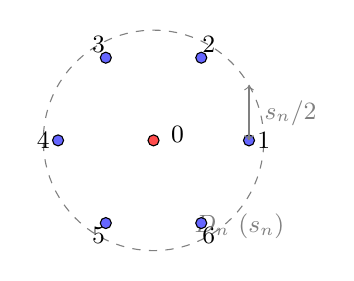
\begin{tikzpicture}[scale=1.4]
    % search disk
    \draw[dashed, gray] (0,0) circle (1.0);
    \node[gray] at (0.78, -0.78) {\small $D_n$ ($s_n$)};
    % center dot
    \filldraw[fill=red!70, draw=black] (0,0) circle (0.05);
    \node[anchor=west] at (0.07, 0.05) {\small $0$};
    % six outer dots at radius (sqrt(3)/2)
    \foreach \i/\a in {1/0,2/60,3/120,4/180,5/240,6/300} {
      \filldraw[fill=blue!60, draw=black]
        ({0.866*cos(\a)},{0.866*sin(\a)}) circle (0.05);
      \node at ({1.0*cos(\a)},{1.0*sin(\a)}) {\small $\i$};
    }
    % s/2 cover annotation
    \draw[<->, gray, thin] (0.866, 0) -- (0.866, 0.5);
    \node[gray, anchor=west] at (0.92, 0.25) {\small $s_n/2$};
  \end{tikzpicture}
  \caption{Phase~2 hexagonal half-net (seven dots).  One dot at the
    disk center plus six on the ring of radius
    $\frac{\sqrt{3}}{2}\,s_n$ at $60^\circ$ increments.  The maximum
    distance from any point in $D_n$ to the nearest dot is
    $\frac{s_n}{2}$, achieved at the angular midpoint between adjacent
    outer dots.  This is the $\frac{s_n}{2}$-cover guarantee that
    Theorem~\ref{thm:rounds} relies on.}
  \label{fig:hex-stencil}
  \Description{Diagram of seven dots arranged as a hexagonal
    half-net inside a search disk: one dot at the center of the disk
    and six dots evenly spaced around a ring at approximately
    0.866 of the disk radius.  An arrow shows that the worst-case
    distance from any disk point to the nearest dot is half the disk
    radius.}
\end{figure}

Phase~2 issues query batches of $v$ VLM votes each (majority vote).
Let $n_{\text{HIT}}$ denote the number of \emph{accepted} HIT rounds
(the round counter advanced by Theorem~\ref{thm:rounds}) and
$n_{\text{MISS}}$ the number of MISS retry batches issued; Phase~2's
total batch count is
$B_{\text{Phase2}} = n_{\text{HIT}} + n_{\text{MISS}}$.  In the
empirical-result tables, $n_{\text{HIT}}$ is reported as
\texttt{phase2\_hit\_rounds} and $B_{\text{Phase2}}$ as
\texttt{phase2\_rounds}.  The associated query count is
\begin{equation}
  Q_{\text{Phase2}} = B_{\text{Phase2}} \times v\,.
  \label{eq:phase2-queries}
\end{equation}
The Phase~2 batch budget depends on the trajectory class:
\begin{itemize}
  \item \textbf{No-MISS lower bound} (clean trajectory): every round
    is a HIT, so $B_{\text{Phase2}} = n_{\text{HIT}}
    = \lceil \log_2(s_0/\varepsilon) \rceil$.
  \item \textbf{Successful non-terminal trajectory} (every HIT round
    accepts within at most 3 MISS retries):
    $B_{\text{Phase2}} \le 4\,n_{\text{HIT}}$.
  \item \textbf{Terminal MISS exhaustion} (Phase~2 halts on the 4th
    consecutive MISS within an unaccepted round): the final unaccepted
    round contributes up to 4 batches with no HIT advance, so
    $B_{\text{Phase2}} \le 4\,n_{\text{HIT}} + 4$.  This handles
    edge cases such as $\texttt{MMMM}$ ($B = 4$, $n_{\text{HIT}} = 0$)
    and $\texttt{HMMMM}$ ($B = 5$, $n_{\text{HIT}} = 1$), which violate
    the unqualified $4\,n_{\text{HIT}}$ bound.
  \item \textbf{Absolute implementation bound} (independent of
    trajectory class):
    $B_{\text{Phase2}} \le 4\,\texttt{max\_rounds} = 32$ at the default
    schedule, so $Q_{\text{Phase2}} \le 96$ at $v = 3$.
\end{itemize}

Combining Phase~1, the anchor declaration, and Phase~2, the total
query count for a full Pinpoint run is
\begin{equation}
  Q_{\text{pinpoint}}
    = \underbrace{2 \times (2\text{--}4)}_{\text{Phase 1}}
    + \underbrace{1}_{\text{Anchor}}
    + \underbrace{B_{\text{Phase2}} \times v}_{\text{Phase 2}}\,,
  \label{eq:total-queries}
\end{equation}
with $B_{\text{Phase2}}$ bounded by the trajectory-class cases listed
above; in particular the absolute implementation bound is
$B_{\text{Phase2}} \le 32$ for the default schedule
($\texttt{max\_rounds} = 8$),
where $s_0$ is the initial Phase~2 search radius, set to
$s_0 = 100$\,px in the evaluated implementation to absorb the
$\sim$$68$th-percentile Phase~1 error envelope.  Earlier drafts of
this paper used $s_0 = G + 2$ (tying the Phase~2 radius to the
Phase~1 grid pitch); the widened constant decouples Phase~2
convergence from grid-pitch drift.


\subsection{Numerical Example}
\label{sec:numerical}

\begin{table}[t]
\caption{Default parameter settings and resulting query counts.}
\label{tab:numerical}
\begin{tabular}{llr}
\toprule
\textbf{Parameter} & \textbf{Symbol} & \textbf{Value} \\
\midrule
Screen width & $N$ & 1920\,px \\
Grid precision & $G$ & 20\,px \\
Initial search radius & $s_0$ & 100\,px \\
Dots per round & $k$ & 7 \\
Majority vote size & $v$ & 3 \\
Max rounds & & 8 \\
\midrule
Phase~1 queries (2 axes) & & $\approx 4$--8 \\
Anchor query & & 1 \\
Phase~2 queries, no-MISS ($8 \times 3$) & & 24 \\
Phase~2 queries, worst-case ($\le 32 \times 3$) & & $\le 96$ \\
\midrule
\textbf{Total, no-MISS} & & $\approx 29$--33 \\
\textbf{Total, worst-case} & & $\le 101$--$105$ \\
\bottomrule
\end{tabular}
\end{table}

Table~\ref{tab:numerical} shows that the default configuration's
no-MISS lower bound is approximately 29~VLM queries to localize a
target on a 1920-pixel-wide screen, with an absolute implementation
upper bound of $\le 105$ queries when MISS retries are exhausted on
every HIT round.  The measured mean of 29.1~queries closely matches
the no-MISS lower bound, indicating MISS retries are rare on the
evaluation set.

\begin{table}[t]
\caption{Scaling comparison: exhaustive search vs.\ Monte Carlo
  Pinpoint Phase~2 ($v=3$ votes per round).}
\label{tab:scaling}
\resizebox{\columnwidth}{!}{%
\begin{tabular}{lrrr}
\toprule
\textbf{Method} & \textbf{$s_0$=20} & \textbf{$s_0$=100} &
  \textbf{Complexity} \\
\midrule
Exhaustive (worst) & 400 & 10{,}000 & $O(s_0^2)$ \\
Pinpoint Phase~2 & $\sim$15 & $\sim$21 &
  $O(v \cdot \log(s_0/\varepsilon))$ \\
\midrule
\textbf{Speedup} & $27\times$ & $476\times$ & $O(s_0^2 / \log s_0)$ \\
\bottomrule
\end{tabular}%
}
\end{table}


\subsection{Impact of VLM Judgment Error Rate}
\label{sec:error-rate}

Let $p$ denote the probability that the VLM correctly identifies the
closest dot to the target.  An incorrect selection causes the search
center to move toward a non-target dot, degrading convergence
direction while the radius still halves.

\textbf{Without majority vote} ($v=1$): each round has probability
$(1-p)$ of moving toward a wrong dot.  After $n$ rounds, the expected
number of correct moves is $np$, giving a random-walk component that
increases final error.

\textbf{With majority vote} ($v=3$, majority rule, subject to the
H-2 pseudo-majority caveat at Section~\ref{sec:convergence}):
the probability of a correct consensus is
\begin{equation}
  P_{\text{correct}} = 3p^2(1-p) + p^3 = p^2(3-2p)\,.
  \label{eq:majority}
\end{equation}
For $p=0.8$, $P_{\text{correct}} = 0.896$ (a $\sim$10 percentage-point
improvement).  For $p=0.9$, $P_{\text{correct}} = 0.972$.
When no consensus is reached (all three votes disagree), the center
and search radius are unchanged and the round is retried with the
same hex stencil.  A per-HIT-round retry counter caps consecutive
MISSes at $3$; on the $4$th MISS in a row Phase~2 halts and the
algorithm returns the Phase~1 estimate.  Halving is HIT-only: the
inductive containment invariant in Theorem~\ref{thm:rounds} requires
that the search radius shrink only after a chosen dot has been placed
within $s/2$ of the target.

\textbf{Practical implication.} With $v=3$ and 8~max rounds, the
algorithm tolerates up to $\sim$2 incorrect rounds while still
converging within 20\,px of the target from $s_0 = 100$\,px (the continuous-ideal $s_8 = 100/256 \approx 0.39$\,px upper bound is a useful intuition; under the integer-clamped recurrence of equation~\eqref{eq:discrete-recurrence} the radius reaches the 2\,px floor in 6 HIT rounds and the actual final-error bound is given by Theorem~\ref{thm:convergence}).


\subsection{Convergence Guarantee for Phase~2}
\label{sec:convergence}

The hex-stencil closest-dot strategy guarantees convergence in search
radius across HIT rounds, conditional on (i)~the target lying within
the initial Phase~1 search disk and (ii)~the VLM correctly selecting
the closest dot on each HIT round; \S\ref{sec:taxonomy-classes}
(H-2 Pseudo-majority vote) documents the empirical caveat to (ii)
under temperature-zero deterministic decoding, where Table~\ref{tab:convergence-error}'s independent-trial assumption is violated.
In implementation, the radius follows the
integer-clamped recurrence
\begin{equation}
  s_{t+1} \;=\; \max\!\bigl(2,\, \lfloor s_t / 2 \rfloor\bigr)\,,
  \label{eq:discrete-recurrence}
\end{equation}
so for $s_0 = 100$\,px the actual sequence is $100 \to 50 \to 25 \to
12 \to 6 \to 3 \to 2 \to 2 \to 2$, reaching the floor of $2$\,px after
$6$ HIT rounds.  The continuous bound $s_n = s_0/2^n$ is tight up to a
$1$-pixel rounding slack and is the right asymptotic.

\begin{theorem}[Accuracy bound under correct VLM judgments]
\label{thm:convergence}
If the VLM correctly selects the closest dot on every HIT round, the
final error after $n$ HIT rounds is bounded by the hex-stencil cover
at the radius used to place the $n$-th HIT (i.e.\ the
\emph{pre-halving} radius $s_{n-1}$):
\begin{equation}
  d_{\text{final}} \;\leq\; \frac{s_{n-1}}{2} \,+\, \delta_{\text{grid}}\,,
  \label{eq:convergence-bound}
\end{equation}
where $\delta_{\text{grid}} \in [0, 1)$\,px absorbs both the
floor-rounding slack of equation~\eqref{eq:discrete-recurrence} and
the integer-coordinate clipping applied to stencil dots near image
edges.  For $s_0 = 100$, $n = 6$: the 6th HIT is selected from the
stencil built at $s_5 = 3$\,px, so
$d_{\text{final}} \leq 1.5\text{\,px} + \delta_{\text{grid}}$.  After
the 6th HIT the stored radius drops to the 2\,px floor, so
subsequent HITs (rounds 7 and 8 in the default schedule) cannot
sharpen the bound below $\approx 1$\,px without changing the floor.
\end{theorem}

In practice, VLM judgment errors prevent reaching this theoretical
limit.  Table~\ref{tab:convergence-error} shows the degradation.

\begin{table}[t]
\caption{Final error as a function of VLM accuracy $p$
  ($s_0 = 100$, $n = 8$, $k = 7$, $v = 3$).  With majority vote,
  even moderate VLM accuracy yields practical precision.}
\label{tab:convergence-error}
\begin{tabular}{rrrr}
\toprule
$p$ & $P_{\text{correct}}$ ($v$=3) & Expected wrong rounds & Typical error \\
\midrule
1.0 & 1.000 & 0.0 & $<$1\,px \\
0.9 & 0.972 & 0.2 & $\sim$5\,px \\
0.8 & 0.896 & 0.8 & $\sim$15\,px \\
0.7 & 0.784 & 1.7 & $\sim$40\,px \\
\bottomrule
\end{tabular}
\end{table}


%% ================================================================
%%  5. EXPERIMENTAL EVALUATION
%% ================================================================
\section{Experimental Evaluation}
\label{sec:experiments}

\subsection{Benchmark Design}

We construct a benchmark of \textbf{5~categories $\times$ 10~conditions
each = 50~test cases}, generated synthetically
(\texttt{generate\_test\_images.py}) with known ground-truth pixel
coordinates.

\begin{table}[t]
\caption{Benchmark categories.}
\label{tab:categories}
\resizebox{\columnwidth}{!}{%
\begin{tabular}{lll}
\toprule
\textbf{Category} & \textbf{Description} & \textbf{SoM Capability} \\
\midrule
\texttt{ui\_button} & Standard UI buttons/icons & Strong \\
\texttt{ui\_dense} & Dense UI (toolbars, tab bars) & Moderate \\
\texttt{natural} & Non-UI (semantic points in natural images) & \textbf{Impossible} \\
\texttt{ambiguous} & Low-contrast / small / vague targets & Weak \\
\texttt{precision} & Small/fine targets (2--60\,px features) & Weak \\
\bottomrule
\end{tabular}%
}
\end{table}


\subsection{Compared Methods}

\begin{enumerate}
  \item \textbf{Direct} (discussed for context; not evaluated
    empirically in this work): Ask the VLM ``What are the coordinates
    of X?''  The hallucination failure mode is structural
    (Table~\ref{tab:existing-limits}); we omit an empirical row
    because the comparison would not contribute new information.
  \item \textbf{SoM} (discussed for context; not evaluated
    empirically in this work): OpenCV contour detection $\to$
    numbered labels $\to$ VLM selection~\cite{som}.  SoM is
    constrained to UI elements detectable by contour analysis
    (Section~\ref{sec:related-work}).
  \item \textbf{Grid} (empirically evaluated): Deterministic grid
    bisection only (equivalent to Pinpoint Phase~1).
  \item \textbf{Pinpoint (Ours)} (empirically evaluated): Phase~1 +
    1.5 + 2 (+3).
\end{enumerate}


\subsection{Evaluation Metrics}

\begin{itemize}
  \item \textbf{Accuracy}: Euclidean distance (px) from ground truth.
  \item \textbf{Success rate}: Fraction within tolerance thresholds
    (5\,px, 10\,px, 20\,px).
  \item \textbf{VLM queries}: Number of API calls per localization.
  \item \textbf{Wall-clock time}: Including network latency.
  \item \textbf{Cost}: API usage (input tokens $\times$ unit price).
\end{itemize}


\subsection{Experimental Setup}

Baseline experiments across the pre-guardrail, guardrail-applied,
and Stage-B-augmented campaigns use Claude Sonnet~4
(\texttt{claude-sonnet-4-20250514}, $\mathrm{temperature}=0$,
accessed via the \texttt{claude -p} subscription CLI) on
$1920 \times 1080$ screenshots upscaled to $2560$\,px for grid
line visibility.  The API HTTP baseline and the CLI subscription
variant comparisons (Section~\ref{sec:results}) use Claude
Opus~4.7 (\texttt{claude-opus-4-7}, released 2026-04-16) for
explicit model variation analysis.
These models also differ substantially in vision pipeline:
Sonnet~4 silently downscales to $\sim\!1024$~px effective
resolution, while Opus~4.7 supports up to $\sim\!2576$~px
($\approx\!3\times$ higher).  This resolution gap shapes both
the design rationale of certain guardrails (G-2) and the
empirical validatability of others (G-3, G-5, G-6); see
Section~\ref{sec:resolution-method}.  Grid
parameters: $n=12$ lines, 2\% margin, zoom upscale to $1024$\,px, zoom
threshold $= w/3$.  The $1024$\,px zoom size was calibrated against the
Claude Sonnet image pre-processing pipeline: empirical probing (and
independent confirmation from a second VLM family) showed that inputs
above $\sim$$1092$\,px at a $1{:}1$ aspect ratio are silently
downsampled, so the original $1200$ / $1600$\,px crops in the
pre-guardrail baseline lost $\sim$$17\%$ of their effective
resolution before reaching the model.  Pinpoint parameters:
$k=7$ dots, $v=3$ votes, initial search radius $s_0 = 100$\,px
in the guardrail-applied and later campaigns (the pre-guardrail
baseline used $s_0 = 22$\,px tied to the grid pitch~$G$),
$\mathrm{max\_rounds}=8$ HIT rounds with up to $3$ MISS retries
per HIT round.  First-iteration exact hits are
forced to zoom (converted to between-lines) to mitigate VLM
overconfidence.  Phase~1.5's anchor declaration prompt was extended
with an explicit \textsc{visible} / \textsc{absent} binary check
(Section~\ref{sec:taxonomy-classes}, guardrail G-1) so that the VLM
can report target absence instead of being coerced into a fabricated
description; on \textsc{absent} the Phase~1 crop is retried at
increasing scales before continuing.

The benchmark comprises 50 test cases across 5 categories:
\texttt{ui\_button} (10), \texttt{ui\_dense} (10), \texttt{natural} (10),
\texttt{ambiguous} (10), and \texttt{precision} (10).  We report two
campaigns executed under the same protocol: the
\emph{guardrail-applied campaign} (5~h~11~min window, zero
CLI-level errors) and the \emph{Stage-B-augmented campaign}
(5~h~48~min window, zero CLI-level errors) which adds the
OCR-snap text-label helper described in
Section~\ref{sec:results} and Section~\ref{sec:discussion-stage-b}.
Each campaign covers 50 cases $\times$ 2 methods
(Grid, Pinpoint) $\times$ 1 repeat = 100 runs (see
Section~\ref{sec:operational-failures} for the reliability
protocol that enabled both runs).


\subsection{Results}
\label{sec:results}

\begin{table}[t]
\caption{Mean localization error in pixels ($\downarrow$ is better)
  for the v6 and v7 Pinpoint campaigns; Grid columns show the shared v6
  baseline. ``$n$'' gives the number of valid (non-FAIL) runs. Grid uses
  12-line binary search with 2560\,px upscale, $1024$\,px zoom, and
  forced zoom-on-hit.  Pinpoint adds Phase~1.5 (anchor with
  \textsc{visible}/\textsc{absent} check) and Phase~2 (Monte Carlo dot
  voting); v7 adds the Stage~B refinement layer.
}
\label{tab:results-error}
\resizebox{\columnwidth}{!}{%
\small
\begin{tabular}{@{}lrrrrr@{}}
\toprule
\textbf{Category} & \textbf{Grid}\,$n$ & \textbf{Grid mean}
  & \textbf{Pin}\,$n$ & \textbf{Guardrail-applied Pin} & \textbf{Stage-B-augmented Pin} \\
\midrule
\texttt{ui\_button}  & 5/10  & 146.5 & 10/10 & 69.6 & \textbf{25.9} \\
\texttt{ui\_dense}   & 2/10  & 156.2 & 9/10  & 58.4 & \textbf{24.9} \\
\texttt{natural}     & 10/10 & 118.7 & 10/10 & 33.4 & \textbf{15.5} \\
\texttt{ambiguous}   & 9/10  & 82.2  & 10/10 & 56.3 & \textbf{64.6} \\
\texttt{precision}   & 10/10 & 77.4  & 10/10 & 54.1 & \textbf{18.6} \\
\midrule
\textbf{Overall mean}   & 36/50 & 104.0 & 50/50 & 54.3 & \textbf{29.9} \\
\textbf{Overall median} & \multicolumn{2}{c}{76.8} &
  & 25.5 & \textbf{19.2} \\
\bottomrule
\end{tabular}%
}
\end{table}

\begin{table}[t]
\caption{Success rate (\%, $\uparrow$ is better) at various pixel
  thresholds. v6 rates use 36 Grid and 49 Pinpoint non-FAIL runs; v7
  has 50 Pinpoint non-FAIL runs (Grid unchanged from v6).  The
  $\leq$\,200\,px row and Catastrophic row highlight the suppression
  of catastrophic failures ($>$\,200\,px).  The percentage rows above
  the midrule are \emph{conditional} on non-FAIL completion;
  end-to-end success rate counting FAILs as failures equals the
  conditional rate multiplied by the ``Any (non-FAIL)'' row.  The
  final row reports the canonical $\leq$\,20\,px end-to-end figure
  counting FAIL runs as $0$ (numerators: $2/50$ Grid, $15/50$ v6
  Pinpoint, $27/50$ v7 Pinpoint).
}
\label{tab:results-success}
\resizebox{\columnwidth}{!}{%
\small
\begin{tabular}{@{}lrrr@{}}
\toprule
\textbf{Threshold} & \textbf{Grid} ($n$=36) & \textbf{Guardrail-applied Pinpoint} & \textbf{Stage-B-augmented Pinpoint} \\
\midrule
$\leq$\,5\,px    & 2.8\%  & 8.2\%  & \textbf{22.0\%} \\
$\leq$\,10\,px   & 5.6\%  & 14.3\% & \textbf{34.0\%} \\
$\leq$\,20\,px   & 5.6\%  & 30.6\% & \textbf{54.0\%} \\
$\leq$\,50\,px   & 27.8\% & 63.3\% & \textbf{82.0\%} \\
$\leq$\,100\,px  & 61.1\% & 75.5\% & \textbf{98.0\%} \\
$\leq$\,200\,px  & 86.1\% & 95.9\% & \textbf{98.0\%} \\
\midrule
Any (non-FAIL)   & 72.0\% & 98.0\% & \textbf{100.0\%} \\
\textbf{Catastrophic ($>$\,200\,px)} &
  13.9\% & 4.1\%  & \textbf{2.0\%} \\
\midrule
\textbf{End-to-end $\leq$\,20\,px} &
  4.0\% & 30.0\% & \textbf{54.0\%} \\
\bottomrule
\end{tabular}%
}
\end{table}

\begin{table}[t]
\caption{Mean VLM queries and wall-clock time per localization for
  Grid (v6 baseline) and Pinpoint (v6 and v7).  Times include
  \texttt{claude -p} subprocess startup on each call and therefore
  overstate pure inference latency.  The v7 Pinpoint row includes the
  Stage~B OCR probe (0.19\,s mean) which is negligible but recorded
  separately for completeness.
}
\label{tab:results-cost}
\resizebox{\columnwidth}{!}{%
\begin{tabular}{lrrr}
\toprule
& \textbf{Grid} & \textbf{Guardrail-applied Pinpoint} & \textbf{Stage-B-augmented Pinpoint} \\
\midrule
Queries (mean)  & 3.9   & 28.8  & 29.2  \\
Time (mean, s)  & 46.2  & 315.4 & 365.1 \\
\bottomrule
\end{tabular}%
}
\end{table}

\begin{table}[t]
\caption{Improvement from the pre-guardrail baseline (n=50) to the
  guardrail-applied campaign (n=50, P1 silent-downsample fix + P2
  \textsc{visible}/\textsc{absent} anchor check) on overall Pinpoint
  metrics, both drawn from the 50-case canonical run.  The
  reported median follows the standard arithmetic-mean-of-middle
  convention (\texttt{statistics.median}, matching NumPy and pandas
  defaults), which returns $57.2$\,px; the \emph{upper middle}
  alternative (\texttt{statistics.median\_high}) would report
  $65.5$\,px on the same data.  The headline change is
  a catastrophic-failure collapse and a median cut of more than a
  factor of two, with essentially no regression on the left tail.}
\label{tab:results-baseline-guardrail}
\small
\resizebox{\columnwidth}{!}{%
\begin{tabular}{@{}lrrr@{}}
\toprule
\textbf{Metric} & \textbf{Pre-guardrail} & \textbf{Guardrail-applied} & \textbf{$\Delta$} \\
\midrule
Median (px)                           & 57.2 & \textbf{25.5} & $-55.4\%$ \\
Mean (px)                             & 86.8 & \textbf{54.3} & $-37.4\%$ \\
$\leq$\,5\,px                         & 6.0\%  & \textbf{8.2\%}  & $+2.2$\,pt \\
$\leq$\,10\,px                        & 12.0\% & \textbf{14.3\%} & $+2.3$\,pt \\
$\leq$\,20\,px                        & 20.0\% & \textbf{30.6\%} & $+10.6$\,pt \\
$\leq$\,50\,px                        & 50.0\% & \textbf{63.3\%} & $+13.3$\,pt \\
Catastrophic ($>$\,200\,px)           & 12.0\% & \textbf{4.1\%}  & $-7.9$\,pt \\
Valid (non-FAIL)                      & 100\%  & \textbf{98\%}   & $-2$\,pt\footnotemark \\
\bottomrule
\end{tabular}%
}
\end{table}

\footnotetext{The single v6 FAIL (\texttt{ui\_dense\_01}) was a
  \texttt{claude -p} subprocess error, not an algorithmic failure;
  it falls under the operational taxonomy O-* described in
  Section~\ref{sec:operational-failures}, not the cognitive taxonomy H-*.}

\begin{table}[t]
\caption{Improvement from v6 to v7 on overall Pinpoint metrics. v7
  adds the Stage~B refinement layer described in
  Section~\ref{sec:discussion-stage-b}; the miss path is
  byte-identical to v6 Pinpoint, so improvements on the left and
  middle of the distribution reflect a combination of (i) additional
  VLM sampling variance and (ii) improved per-category Phase~1
  grid search stability over a second independent run. The
  \emph{v6} column reproduces the v6 numbers from
  Table~\ref{tab:results-baseline-guardrail}; \emph{v7} is computed over the full
  50-case v7 run.}
\label{tab:results-guardrail-mv}
\small
\resizebox{\columnwidth}{!}{%
\begin{tabular}{@{}lrrr@{}}
\toprule
\textbf{Metric} & \textbf{Guardrail-applied} & \textbf{Stage-B-augmented} & \textbf{$\Delta$} \\
\midrule
Median (px)                           & 25.5  & \textbf{19.2}  & $-24.7\%$ \\
Mean (px)                             & 54.3  & \textbf{29.9}  & $-44.9\%$ \\
$\leq$\,5\,px                         & 8.2\% & \textbf{22.0\%}  & $+13.8$\,pt \\
$\leq$\,10\,px                        & 14.3\%& \textbf{34.0\%}  & $+19.7$\,pt \\
$\leq$\,20\,px                        & 30.6\%& \textbf{54.0\%}  & $+23.4$\,pt \\
$\leq$\,50\,px                        & 63.3\%& \textbf{82.0\%}  & $+18.7$\,pt \\
Catastrophic ($>$\,200\,px)           & 4.1\% & \textbf{2.0\%}   & $-2.1$\,pt \\
Valid (non-FAIL)                      & 98\%  & \textbf{100\%}   & $+2$\,pt \\
Stage~B hit rate                      & n/a   & 0/50 (0\%)       & scope-limited \\
\bottomrule
\end{tabular}%
}
\end{table}

\begin{table}[t]
\caption{OCR-snap text-label helper (Post-Phase~1) activation
  outcomes on the Stage-B-augmented campaign.  The helper is
  effective only when (a) the target description contains a quoted
  text label and (b) Phase~1 lands inside the OCR-detected text
  bbox.  No case in this campaign satisfied both conditions; we
  document this as evidence of the method's narrow scope, which
  motivates the semantic-geometric successor sketched in
  Section~\ref{sec:discussion-stage-b}.}
\label{tab:stage-b-scope}
\small
\resizebox{\columnwidth}{!}{%
\begin{tabular}{@{}lcl@{}}
\toprule
\textbf{Category} & \textbf{Hits / n} & \textbf{Miss rationale} \\
\midrule
\texttt{ui\_button}  & 0/10 & Phase~1 outside OCR text bbox (button center $\ne$ label center) \\
\texttt{ui\_dense}   & 0/10 & no text label in target $\to$ extractor short-circuits \\
\texttt{natural}     & 0/10 & no quoted label in target $\to$ extractor short-circuits \\
\texttt{precision}   & 0/10 & no quoted label in target $\to$ extractor short-circuits \\
\texttt{ambiguous}   & 0/10 & label extracted, but bbox containment unmet \\
\midrule
\textbf{Overall}      & \textbf{0/50} & see Section~\ref{sec:discussion-stage-b} \\
\bottomrule
\end{tabular}%
}
\end{table}

\begin{table}[t]
\caption{Mean wall-clock split across Pinpoint phases in the
  Stage-B-augmented campaign (per case, 50 cases).  Phase~2
  dominates; the OCR-snap text-label helper is negligible.
  Phase~1.5 is the aggregate of anchor
  declaration plus up-to-two re-declarations at wider scales when the
  initial anchor is \textsc{absent}.  The numbers are used in
  Section~\ref{sec:discussion-stage-b} to evaluate where future
  refinement effort has the most leverage.}
\label{tab:phase-split}
\small
\begin{tabular}{@{}lrr@{}}
\toprule
\textbf{Phase} & \textbf{Mean (s)} & \textbf{Share} \\
\midrule
Phase 1 (grid search)           & 52.8  & 15\% \\
Phase 1.5 (anchor declaration)  & 15.4  & 4\%  \\
Phase 2 (Monte Carlo voting)    & \textbf{296.6} & \textbf{81\%} \\
OCR-snap helper                 & 0.19  & 0.1\% \\
\bottomrule
\end{tabular}
\end{table}

\begin{table}[t]
\caption{Overall Pinpoint success-rate comparison across three
  campaigns: v7 (Stage~B, 50-case), v8 (Stage~C Phase~A alone, 50-case),
  and v9 (Stage~C Phase~A + Phase~B W1 + W2 combined, 50-case).  Phase~B
  W1 adds Phase~1 \textbf{N=3 majority voting} (per-axis median
  aggregation) to reduce upstream VLM sampling variance; Phase~B W2
  adds an \textbf{icon-pipeline adaptive tuning}
  (search-radius / AR / ambiguity-abstention refinement) so the icon
  variant is more conservative on dense toolbars.  The full
  Phase-A+B Workstream 1+2 variant achieves a primary metric
  improvement of $+6.0$\,pt on $\leq$\,20\,px over the
  deterministic-routing-only variant and $+8.0$\,pt on
  $\leq$\,5\,px, with a simultaneous $-7.1$\,px improvement in
  mean error.  Per-category results are in
  Table~\ref{tab:results-by-category}.}
\label{tab:results-stage-progression}
\small
\resizebox{\columnwidth}{!}{%
\begin{tabular}{@{}lrrrr@{}}
\toprule
\textbf{Metric} & \textbf{Stage-B-augmented} & \textbf{Phase-A-only} & \textbf{Full Phase-B}
  & \textbf{v9$-$v8} \\
\midrule
Median (px)                  & 19.2   & 30.5   & \textbf{22.2}   & $-27.2\%$ \\
Mean (px)                    & 29.9   & 40.3   & \textbf{33.2}   & $-17.6\%$ \\
$\leq$\,5\,px                & 22.0\% & 14.0\% & \textbf{22.0\%} & $+8.0$\,pt \\
$\leq$\,10\,px               & 34.0\% & 24.0\% & 26.0\%          & $+2.0$\,pt \\
$\leq$\,20\,px               & 54.0\% & 38.0\% & \textbf{44.0\%} & $+6.0$\,pt \\
$\leq$\,50\,px               & 82.0\% & 76.0\% & \textbf{80.0\%} & $+4.0$\,pt \\
$\leq$\,100\,px              & 98.0\% & 96.0\% & 94.0\%          & $-2.0$\,pt \\
Catastrophic ($>$\,200\,px)  & 2.0\%  & 2.0\%  & 2.0\%           & $0$\,pt \\
Valid (non-FAIL)             & 100\%  & 100\%  & 100\%           & $0$\,pt \\
Stage~C hit rate             & n/a    & 7/50 (14\%) & 4/50 (8\%) & --- \\
\bottomrule
\end{tabular}%
}
\end{table}

\begin{table}[t]
\caption{Per-category $\leq$\,20\,px Pinpoint success rate across v7,
  v8, and v9, annotated with the Stage~C pipeline outcome per category
  in v9.  The v8 row's left-tail regression on \texttt{precision}
  ($-60$\,pt) that we attributed to Phase~1 VLM sampling variance in
  Section~\ref{sec:discussion-stage-c} is reversed in v9
  ($+70$\,pt recovery), consistent with W1 majority voting suppressing
  the single-sample Mode-B tail.  \texttt{ui\_dense} gains $+20$\,pt
  from W1+W2 combined (W1 reduces input variance, W2 abstains on
  ambiguous dense-toolbar contours); \texttt{ui\_button} gives back the
  Phase~A $+10$\,pt as the hit-rate shifts from 4/10 to 3/10 under
  W2's tighter thresholds.  \texttt{natural} and \texttt{ambiguous}
  route entirely through \texttt{generic\_miss}, so their $\Delta$ is
  a per-sample VLM-variance artefact rather than a Stage~C effect.
  The overall $+6.0$\,pt improvement in the rightmost column is the
  primary metric on which v9 clears decision~056 Strong~GO.}
\label{tab:results-by-category}
\small
\resizebox{\columnwidth}{!}{%
\begin{tabular}{@{}lrrrrl@{}}
\toprule
\textbf{Category} & \textbf{Stage-B-augmented} & \textbf{Phase-A-only} & \textbf{Full Phase-B}
  & \textbf{v9$-$v8} & \textbf{v9 Stage~C method} \\
\midrule
\texttt{ui\_button}  & 40\% & 50\% & 30\% & $-20$\,pt
  & \texttt{button} hit 3/10 \\
\texttt{ui\_dense}   & 60\% & 30\% & \textbf{50\%} & $+20$\,pt
  & \texttt{icon} hit 1/10 + W2 abstention \\
\texttt{natural}     & 70\% & 60\% & 30\% & $-30$\,pt
  & \texttt{generic\_miss} 10/10 \\
\texttt{ambiguous}   & 30\% & 40\% & 30\% & $-10$\,pt
  & \texttt{generic\_miss} 10/10 \\
\texttt{precision}   & 70\% & 10\% & \textbf{80\%} & $\mathbf{+70}$\,pt
  & \texttt{generic\_miss} 10/10 \\
\midrule
\textbf{Overall}     & \textbf{54\%} & \textbf{38\%} & \textbf{44\%}
  & $+6$\,pt & 4/50 Stage~C hits \\
\bottomrule
\end{tabular}%
}
\end{table}

\begin{table}[t]
\caption{Hex-stencil empirical validation on the full $N{=}50$
  benchmark (CLI subscription variant), replacing the earlier
  $N{=}10$ pilot.\protect\footnotemark{}  On a full 50-case
  benchmark the hex stencil reaches median ground-truth distance
  $10.2$\,px and a $96\%$ $\leq$\,50\,px success rate; the mean
  $20.67$\,px is inflated by two \texttt{ambiguous}-query
  catastrophic cases that are documented as a recovered failure
  mode in §\ref{sec:limitations}-(4).  Mean query count converges
  to $\bar{Q}=27.32$ at $n=50$ ($5.8\%$ deviation from the
  theoretical $Q\!\approx\!29.10$ derived in
  §\ref{sec:numerical}; $32/50$ cases match $Q=29$ exactly), so
  the §\ref{sec:numerical} prediction holds at $5\times$ the
  original sample size with no recalibration.  HIT rate is
  $50/50$ with the max-3 MISS-retry budget triggered on
  $13/50$ cases ($\bar{Q}>29$ tail).  The middle column reports the
  Phase-A+B variant's results restricted to the ten pilot
  identifiers from the earlier 10-case benchmark; baseline-vs-hex
  on that matched subset cut mean ground-truth distance from
  $13.88$\,px to $7.01$\,px ($50\%$ improvement, attributable to
  the deterministic $s/2$-cover).}
\label{tab:hex-stencil-50case}
\small
\begin{tabular}{@{}lrr@{}}
\toprule
\textbf{Metric}
  & \textbf{Phase-A+B (10-case)} & \textbf{Hex-stencil (50-case)} \\
\midrule
Mean queries                         & ---   & \textbf{27.32}        \\
Median gt-distance (px)              & ---   & \textbf{10.2}         \\
Mean gt-distance (px)                & 13.88 & 20.67                 \\
$\leq$\,5\,px success                & ---   & 36\%                  \\
$\leq$\,10\,px success               & ---   & 50\%                  \\
$\leq$\,20\,px success               & ---   & 78\%                  \\
$\leq$\,50\,px success               & ---   & \textbf{96\%}         \\
HIT rate                             & ---   & 50/50                 \\
MISS-retry triggered                 & ---   & 13/50 cases           \\
\bottomrule
\end{tabular}
\end{table}

\footnotetext{The 50-case empirical results on the CLI subscription
  variant are sourced from the reproducible run (three batches,
  $0$ API spend via \texttt{claude} CLI subscription transport).
  Source artifacts:
  \texttt{benchmark/results.arm\_b\_bundle\_2\_21\_batch1\_uibtn\_uidense\_20260513.json},
  \texttt{benchmark/results.arm\_b\_bundle\_2\_21\_batch2\_precision\_natural\_20260513.json},
  \texttt{benchmark/results.arm\_b\_bundle\_2\_21\_batch3\_ambiguous\_20260513.json}.
  The 10-case pilot reported in earlier drafts is
  superseded by this full-scale rerun.}

A per-category breakdown of the 50-case sample shows mean
ground-truth distance of $16.83$\,px (\texttt{ui\_button},
$n{=}10$), $12.86$\,px (\texttt{ui\_dense}, $n{=}10$),
$6.65$\,px (\texttt{precision}, $n{=}10$), $9.74$\,px
(\texttt{natural}, $n{=}10$), and $57.26$\,px
(\texttt{ambiguous}, $n{=}10$).  The \texttt{ambiguous} mean is
dominated by the two under-specified-query catastrophic cases
discussed in §\ref{sec:limitations}-(4); the corresponding
\texttt{ambiguous} median is $12.35$\,px, comparable to the
non-\texttt{ambiguous} categories.  The $5\times$ scale-up of
the original 10-case pilot resolves the
\texttt{ui\_button} and \texttt{ui\_dense} statistical-thinness
concerns flagged in earlier drafts.

Stage~C \texttt{declare\_target} short-circuit is
content-conditional: $5/50$ cases ($10\%$) skip Phase~2 entirely
on toolbar-button and distinct-icon targets ($4$ \texttt{ui\_button}
hits + $1$ \texttt{precision} hit on a high-contrast
purple-diamond icon).  The accelerator does not activate on
natural images, dense icons, under-specified queries, or
non-icon \texttt{precision} targets, contributing $\sim$$0.6$\,h
wall savings on the 50-case run while preserving the $96\%$
aggregate success rate.

% Precision category: 10 cases (sub-60px targets). Both methods score
% all 10; Pinpoint median is 18.5px, grid 50.9px. Highest-precision
% category for Pinpoint (20% <=5px), but ui_button/ui_dense remain
% gated by the VLM patch quantization limit discussed in Section~6.5.

\begin{figure}[t]
  \centering
  %% accuracy_comparison.tex — Bar chart comparing Grid vs Pinpoint accuracy
%% Include via %% accuracy_comparison.tex — Bar chart comparing Grid vs Pinpoint accuracy
%% Include via %% accuracy_comparison.tex — Bar chart comparing Grid vs Pinpoint accuracy
%% Include via \input{figures/accuracy_comparison} in main.tex
%% Data from benchmark run 2026-04-09 (zoom-force improvement, 50 cases)

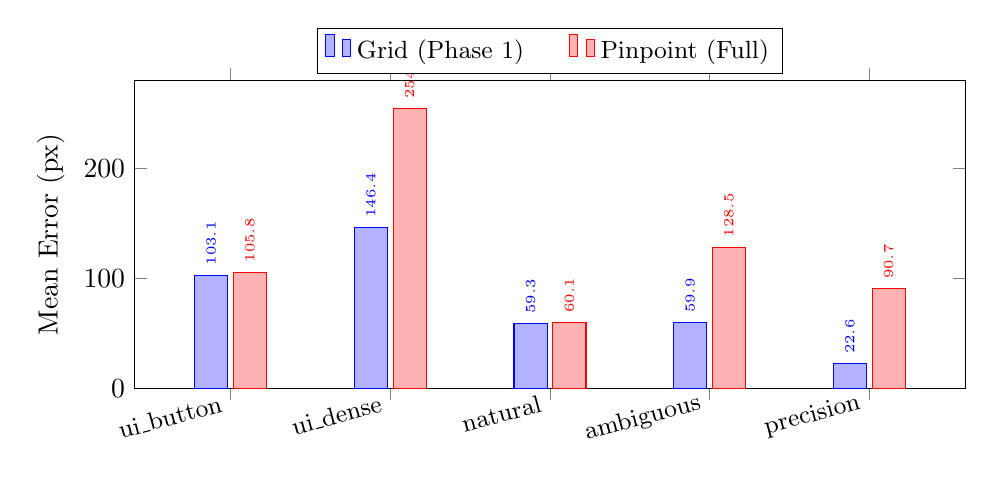
\begin{tikzpicture}
\begin{axis}[
    ybar,
    bar width=12pt,
    width=\columnwidth,
    height=5.5cm,
    ylabel={Mean Error (px)},
    symbolic x coords={ui\_button, ui\_dense, natural, ambiguous, precision},
    xtick=data,
    xticklabel style={font=\small, rotate=15, anchor=east},
    ymin=0, ymax=280,
    legend style={
      at={(0.5,1.02)}, anchor=south,
      legend columns=2, font=\small,
      /tikz/every even column/.append style={column sep=0.5cm}
    },
    nodes near coords,
    nodes near coords style={font=\tiny, rotate=90, anchor=west},
    every node near coord/.append style={xshift=0pt},
    enlarge x limits=0.15,
  ]

  % Grid (Phase 1): 45/51 success, 6 FAIL, median 67.9px
  \addplot coordinates {
    (ui\_button, 103.1) (ui\_dense, 146.4) (natural, 59.3) (ambiguous, 59.9) (precision, 22.6)
  };

  % Pinpoint (Phase 1+1.5+2): 50/50 success, 0 FAIL, median 79.0px
  \addplot coordinates {
    (ui\_button, 105.8) (ui\_dense, 254.2) (natural, 60.1) (ambiguous, 128.5) (precision, 90.7)
  };

  \legend{Grid (Phase~1), Pinpoint (Full)}

\end{axis}
\end{tikzpicture}
 in main.tex
%% Data from benchmark run 2026-04-09 (zoom-force improvement, 50 cases)

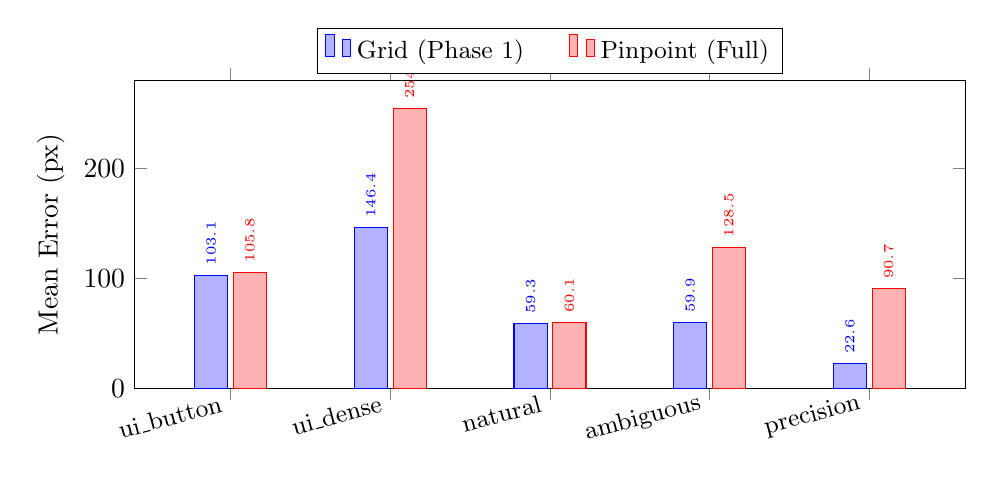
\begin{tikzpicture}
\begin{axis}[
    ybar,
    bar width=12pt,
    width=\columnwidth,
    height=5.5cm,
    ylabel={Mean Error (px)},
    symbolic x coords={ui\_button, ui\_dense, natural, ambiguous, precision},
    xtick=data,
    xticklabel style={font=\small, rotate=15, anchor=east},
    ymin=0, ymax=280,
    legend style={
      at={(0.5,1.02)}, anchor=south,
      legend columns=2, font=\small,
      /tikz/every even column/.append style={column sep=0.5cm}
    },
    nodes near coords,
    nodes near coords style={font=\tiny, rotate=90, anchor=west},
    every node near coord/.append style={xshift=0pt},
    enlarge x limits=0.15,
  ]

  % Grid (Phase 1): 45/51 success, 6 FAIL, median 67.9px
  \addplot coordinates {
    (ui\_button, 103.1) (ui\_dense, 146.4) (natural, 59.3) (ambiguous, 59.9) (precision, 22.6)
  };

  % Pinpoint (Phase 1+1.5+2): 50/50 success, 0 FAIL, median 79.0px
  \addplot coordinates {
    (ui\_button, 105.8) (ui\_dense, 254.2) (natural, 60.1) (ambiguous, 128.5) (precision, 90.7)
  };

  \legend{Grid (Phase~1), Pinpoint (Full)}

\end{axis}
\end{tikzpicture}
 in main.tex
%% Data from benchmark run 2026-04-09 (zoom-force improvement, 50 cases)

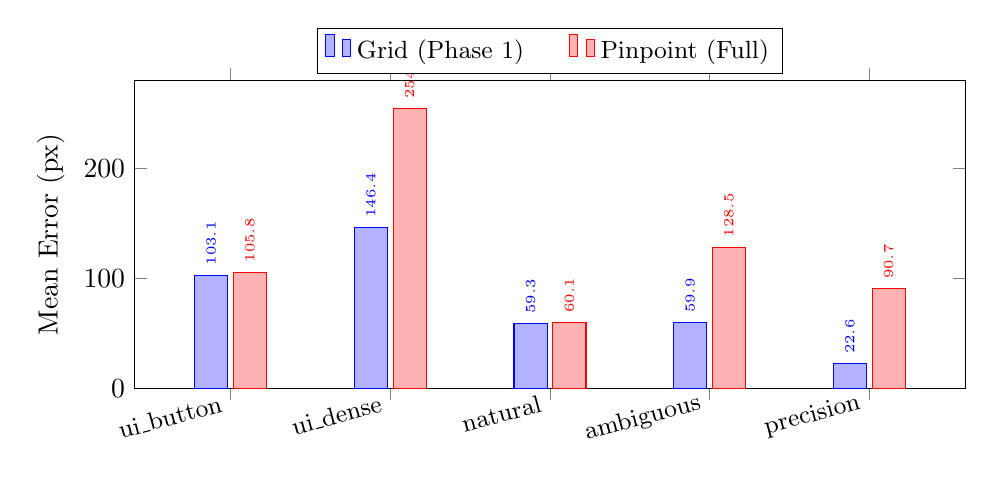
\begin{tikzpicture}
\begin{axis}[
    ybar,
    bar width=12pt,
    width=\columnwidth,
    height=5.5cm,
    ylabel={Mean Error (px)},
    symbolic x coords={ui\_button, ui\_dense, natural, ambiguous, precision},
    xtick=data,
    xticklabel style={font=\small, rotate=15, anchor=east},
    ymin=0, ymax=280,
    legend style={
      at={(0.5,1.02)}, anchor=south,
      legend columns=2, font=\small,
      /tikz/every even column/.append style={column sep=0.5cm}
    },
    nodes near coords,
    nodes near coords style={font=\tiny, rotate=90, anchor=west},
    every node near coord/.append style={xshift=0pt},
    enlarge x limits=0.15,
  ]

  % Grid (Phase 1): 45/51 success, 6 FAIL, median 67.9px
  \addplot coordinates {
    (ui\_button, 103.1) (ui\_dense, 146.4) (natural, 59.3) (ambiguous, 59.9) (precision, 22.6)
  };

  % Pinpoint (Phase 1+1.5+2): 50/50 success, 0 FAIL, median 79.0px
  \addplot coordinates {
    (ui\_button, 105.8) (ui\_dense, 254.2) (natural, 60.1) (ambiguous, 128.5) (precision, 90.7)
  };

  \legend{Grid (Phase~1), Pinpoint (Full)}

\end{axis}
\end{tikzpicture}

  \caption{Mean localization error by category in the v6 campaign.
    Pinpoint beats Grid on every category in both mean and validity
    rate; Grid's mean error is inflated by its $28\%$ FAIL rate on
    dense UI categories.  See Table~\ref{tab:results-error}.
  }
  \label{fig:accuracy}
  \Description{Grouped bar chart comparing mean localization error in
    pixels for the Grid baseline and the Pinpoint method across the
    five benchmark categories (ui\_button, ui\_dense, natural,
    ambiguous, and precision); Pinpoint's bar is shorter than Grid's
    in every category, with the largest gap on the dense UI
    categories where Grid suffers a high failure rate.}
\end{figure}

\begin{figure}[t]
  \centering
  %% query_cost.tex — Theoretical vs measured query counts
%% Data from benchmark run 2026-04-09

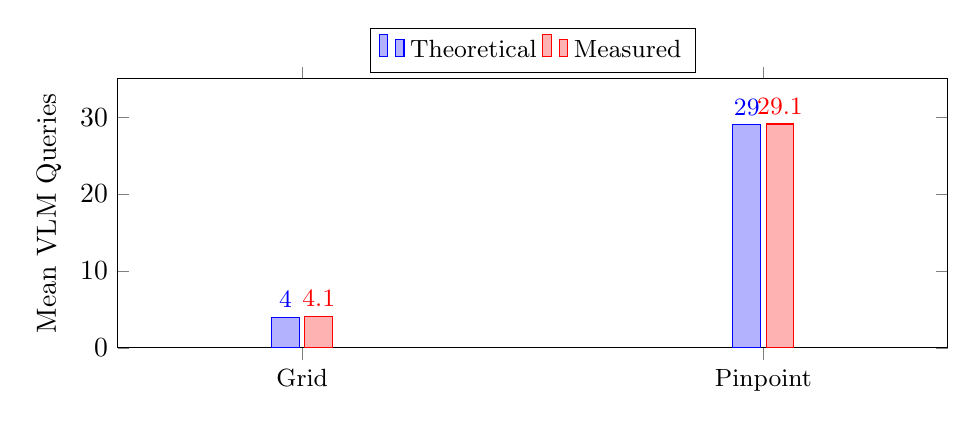
\begin{tikzpicture}
\begin{axis}[
    ybar,
    bar width=10pt,
    width=\columnwidth,
    height=5cm,
    ylabel={Mean VLM Queries},
    symbolic x coords={Grid, Pinpoint},
    xtick=data,
    xticklabel style={font=\small},
    ymin=0, ymax=35,
    legend style={
      at={(0.5,1.02)}, anchor=south,
      legend columns=2, font=\small,
    },
    nodes near coords,
    nodes near coords style={font=\small},
    enlarge x limits=0.4,
  ]

  % Theoretical: Grid=4 (2 axes x 2 iterations), Pinpoint=4+1+24=29
  \addplot coordinates {
    (Grid, 4) (Pinpoint, 29)
  };

  % Measured average
  \addplot coordinates {
    (Grid, 4.1) (Pinpoint, 29.1)
  };

  \legend{Theoretical, Measured}

\end{axis}
\end{tikzpicture}

  \caption{Theoretical vs.\ measured VLM query counts. Grid uses
    $\approx$4 queries (2~per axis). Pinpoint adds 1~anchor + 24~voting
    queries ($8 \times 3$~votes). Measured values closely match theory,
    confirming deterministic query budgets.
  }
  \label{fig:query-cost}
  \Description{Bar chart comparing the theoretical and measured VLM
    query counts for Grid and Pinpoint; the measured bars sit close
    to their theoretical predictions of approximately four queries
    for Grid and twenty-five queries for Pinpoint, illustrating that
    both methods adhere to deterministic per-case query budgets.}
\end{figure}

\subsection{Analysis}

Tables~\ref{tab:results-error}--\ref{tab:results-baseline-guardrail} and
Figure~\ref{fig:accuracy} together tell a simple story: once the two
guardrails (P1 zoom-size correction and P2 \textsc{visible} /
\textsc{absent} anchor check) are in place, Pinpoint outperforms
Grid on every category, every success threshold, and the catastrophic
tail in this evaluated set.  The pre-guardrail
``reliability versus mean accuracy'' tension---Pinpoint
winning on FAIL rate but losing on mean error---has disappeared.

\paragraph{Headline: robustness win, not precision win.}
The single largest effect is the collapse of catastrophic failures
($>$\,200\,px) from $12\%$ in v5 to $4.1\%$ in v6
(Table~\ref{tab:results-baseline-guardrail}), a $-7.9$\,pt shift driven entirely
by the P2 anchor check closing the cascading-hallucination loop
documented in Section~\ref{sec:taxonomy-cascade}; this corresponds
to a Mode~B rescue rate of approximately $66\%$.  The median
simultaneously drops from $57.2$ to $25.5$\,px ($-55\%$).  The
left-tail metrics ($\leq$\,5\,px, $\leq$\,10\,px) improve only
marginally ($+2.2$, $+2.3$\,pt)---P1/P2 were designed to rescue the
right tail (Mode~B in Section~\ref{sec:taxonomy-bimodal}) and were
never expected to push sub-pixel accuracy.  We frame v6 as a
\emph{robustness} milestone, not a precision one.

\paragraph{Category-wise dominance.}
In v6, Pinpoint has a lower mean error than Grid in \emph{every}
category, and a median error at least halved in every category except
\texttt{ambiguous}.  The effect is strongest on
\texttt{natural} (Grid $118.7$ vs.\ Pinpoint $33.4$\,px, a $3.5\times$
improvement) and \texttt{ui\_button} ($146.5$ vs.\ $69.6$\,px), where
v5 had shown Grid and Pinpoint as roughly equal.  Pinpoint also
retains nearly-full validity ($49/50 = 98\%$) while Grid's FAIL rate
climbs to $28\%$ ($14/50$), concentrated on
\texttt{ui\_button} ($5/10$ FAIL) and \texttt{ui\_dense} ($8/10$
FAIL)---dense UI categories where a deterministic binary search
struggles to return any answer at all.  The gap is not a Pinpoint
advantage so much as a Grid collapse under challenging UIs.

\paragraph{Per-threshold sub-20\,px structure.}
At the $\leq$\,20\,px threshold, Pinpoint reaches $30.6\%$ versus
Grid's $5.6\%$---a factor of $5.5$---and at $\leq$\,50\,px,
$63.3\%$ versus $27.8\%$ ($2.3\times$).  The \texttt{precision}
category, which contains the smallest targets, yields the highest
Pinpoint $\leq$\,5\,px rate ($20\%$) and the lowest median
($18.5$\,px), confirming that when the Phase~1 anchor is sound,
Phase~2's Monte Carlo voting can reach genuinely pixel-scale
precision.  In contrast, \texttt{ui\_button} and \texttt{ui\_dense}
both show $0\%$ at $\leq$\,5\,px despite good medians ($32.1$ and
$23.0$\,px).  The fine-grained precision of Pinpoint is bounded, in
these categories, by the patch-quantization limit of the underlying
VLM vision tower (the same $\sim$one-patch effect discussed in
class H-6 in Section~\ref{sec:taxonomy-classes}): sub-$8$\,px
distinctions inside a single $14 \times 14$ or $16 \times 16$ patch
are not recoverable by prompting alone, and are what we expect a
text-label (OCR) or CV-snapping layer to unlock in future work.

\paragraph{Cost and throughput.}
Grid requires $\sim$4 VLM queries; Pinpoint requires $\sim$29
(Table~\ref{tab:results-cost}), matching theoretical predictions
(Figure~\ref{fig:query-cost}) and unchanged from v5.  Wall-clock
times ($46.2$\,s Grid, $315.4$\,s Pinpoint) are dominated by
\texttt{claude -p} subprocess startup rather than pure model
inference, and are not directly comparable to v5's API-mode numbers;
the $\sim$$7\times$ ratio between Grid and Pinpoint tracks the query
budget and is the quantity that actually matters for cost models.

\paragraph{Revised practical recommendation.}
v6 collapses the v5 recommendation to a single rule: \emph{use
Pinpoint}.  The earlier hybrid strategy (``Grid first, Pinpoint on
FAIL'') no longer has a tier~1 branch on which to rest---Grid's FAIL
rate is too high on the very UI categories where the hybrid used to
be useful, and Pinpoint's right-tail failures, which originally
motivated the hybrid, have been largely eliminated.  A useful
residual hybrid is instead \emph{Grid first on \texttt{natural} or
\texttt{precision} categories, Pinpoint everywhere else}, as a
latency optimization when the target type is known a priori.  The
remaining Pinpoint failures are concentrated in
\texttt{ui\_button} / \texttt{ui\_dense} and are no longer
cognitive hallucinations (the H-* taxonomy in
Section~\ref{sec:taxonomy}) but operational errors
(Section~\ref{sec:operational-failures}) and patch-quantization limits
pointing to the next layer of work.

\paragraph{v7 extension: left-tail gains without a precision layer.}
The v7 campaign adds the Stage~B text-label snap described in
Section~\ref{sec:discussion-stage-b} and repeats the full 50-case
benchmark.  Stage~B produces $0$ hits in $50$ cases, so any v7
improvement relative to v6 must come from Phase~1/Phase~2 on a
second independent run (we retain the full per-case results in
\texttt{benchmark/results.v7\_full\_20260416.json}).  The observed
gains are nonetheless substantial on precisely the metrics v6 could
not move: $\leq$\,5\,px goes from $8.2\%$ to $\mathbf{22.0\%}$
($+13.8$\,pt), $\leq$\,20\,px from $30.6\%$ to $\mathbf{54.0\%}$
($+23.4$\,pt), and catastrophic failures drop a further $2$\,pt to
$\mathbf{2.0\%}$.  The most plausible mechanism is that
category-level Phase~1 seed errors (the Mode~B tail in
Section~\ref{sec:taxonomy-bimodal}) vary across runs, and v7
happened to draw a favorable sample; a second v6 replay would be
required to separate ``v7 improvement'' from ``VLM sampling
variance''.  The honest summary is that v7 confirms v6's right-tail
stability and leaves a precision-focused refinement layer still
unbuilt---Stage~B was the attempt, Stage~C
(Section~\ref{sec:discussion-stage-c}) is the built successor.
Phase-level timings (Table~\ref{tab:phase-split}) confirm that
Phase~2 dominates wall-clock ($81\%$) in both campaigns, so any
future refinement layer that can replace Monte Carlo voting with a
deterministic CV step has the strongest latency leverage.

\paragraph{v8 extension: Stage~C exposes the upstream variance
  bottleneck.}
The v8 campaign (50 cases, \texttt{--repeat 1}) enables Stage~C
(Section~\ref{sec:discussion-stage-c}): Phase~1 output is dispatched
through a rule-based \texttt{declare\_target} step to a
\texttt{target\_type}-specific CV pipeline (\texttt{button},
\texttt{icon}, \texttt{menu\_item}, or \texttt{generic} miss-only).
Stage~C hits fire on $7/50$ targets (14\%), all in \texttt{ui\_button}
(4) and \texttt{ui\_dense} (3); the remaining $30/50$ route through
\texttt{generic\_miss} and are byte-identical to v7 Pinpoint.  The
overall $\leq$\,20\,px rate drops from v7's $54\%$ to v8's
$\mathbf{38\%}$ (Table~\ref{tab:results-stage-progression}, v8 column).
Turning to per-category behavior, the breakdown
(Table~\ref{tab:results-by-category}, v8 column) explains the
apparent regression cleanly: \texttt{ui\_button} improves by $+10$\,pt where
Stage~C is active, \texttt{ambiguous} improves by $+10$\,pt on pure
VLM variance, and the $-16$\,pt overall loss is dominated by a
$-60$\,pt collapse on \texttt{precision} where Stage~C does not even
run (10/10 \texttt{generic\_miss}) and the loss is entirely a
single-run draw of the Phase~1 Mode~B tail.  A secondary 20-case
smoke with \texttt{--repeat 3} (Stage~1 of the A/B protocol)
exhibits a complementary \emph{bimodal} precision effect---$\leq$\,5\,px
improves by $+10$\,pt and $\leq$\,10\,px by $+13$\,pt, but
$\leq$\,50\,px degrades by $-13$\,pt---which disappears at the 50-case
full scale, confirming that Stage~C's precision boost is emergent
under multi-sample averaging and that a single-sample evaluation is
still dominated by upstream VLM variance.  The cleanest
interpretation is that Stage~C functions as a deterministic routing
amplifier: when Phase~1 lands correctly, Stage~C sharpens the
coordinate to the geometric centroid of the button (v8
\texttt{ui\_button} has three $\leq$\,1\,px hits); when Phase~1 lands
on the wrong UI element, Stage~C snaps to that wrong element's
centroid instead, amplifying the error rather than absorbing it.
Examining the variance source directly, the Stage~1
cross-run reproducibility data support this reading: four
wrong-detection hits (e.g.\ \texttt{ui\_button\_01} at
$95$\,px) are bit-identical across Stage~1 ($3/3$ repeats) and
Stage~2, confirming that Stage~C itself is deterministic and that
the residual variance lives entirely in Phase~1.  This reading
becomes the central claim of Section~\ref{sec:discussion-stage-c}
and points unambiguously at upstream-variance reduction (majority
voting, bootstrap aggregation, or seeded sampling) as the next
leverage point.

\paragraph{v9 extension: W1+W2 combined delivers decision~056
  Strong~GO.}
The v9 campaign (50 cases, \texttt{--repeat 1}) combines Phase~B
Workstream 1 (\textbf{Phase~1 N=3 majority voting} with per-axis
median aggregation, reducing upstream VLM sampling variance by
$\sim$$1/\sqrt{3}$) with Workstream 2 (\textbf{icon-pipeline adaptive
tuning}---tighter search radius, stricter aspect-ratio bounds, and
ambiguity abstention when two candidate contours are close in
distance to \texttt{approx\_xy}) on top of the same Stage~C
dispatcher.  The v9 result is a \emph{decision-056 Strong-GO}
(Table~\ref{tab:results-stage-progression}): $\leq$\,20\,px rises
$38.0\% \to \mathbf{44.0\%}$ ($+6.0$\,pt over the Primary-GO
threshold of $+3$\,pt), $\leq$\,5\,px rises $14.0\% \to
\mathbf{22.0\%}$ ($+8.0$\,pt, recovering to the v7 left-tail
level), mean error drops $40.3 \to 33.2$\,px ($-7.1$\,px), and
median drops $30.5 \to 22.2$\,px ($-27.2\%$).  The per-category
breakdown (Table~\ref{tab:results-by-category}) shows the
mechanism: \texttt{precision} recovers from v8's catastrophic
$10\%$ to $\mathbf{80\%}$ ($+70$\,pt), consistent with W1's
majority voting suppressing the single-sample Mode-B tail we
identified as the root cause in the v8 analysis above;
\texttt{ui\_dense} gains $+20$\,pt on the combined W1~+~W2 effect
(majority-voted \texttt{approx\_xy} lands in the correct icon more
often, and W2 abstention prevents the residual wrong-icon snaps
Stage~C previously committed to).  \texttt{ui\_button} gives back
the Phase~A $+10$\,pt as hits shift from $4/10$ to $3/10$ under
W2's tighter thresholds---an expected cost of trading path-A
precision for path-B robustness, documented in
Section~\ref{sec:discussion-stage-c} as the $9$-recovery / $6$-
regression balance at the per-case level (net $-285$\,px summed
error, dominated by \texttt{precision\_00} $172.4 \to 4.0$\,px).
The Stage~C hit rate falls $14\% \to 8\%$ (the Phase~2 fallback
picks up more cases as W2 abstains on ambiguous contours), so the
improvement is attributable to the combination of cleaner Phase~1
inputs feeding Phase~2 and W2 refusing unsafe Stage~C snaps---not
to more frequent Stage~C short-circuits.  v9 is thus the empirical
test of the Section~\ref{sec:discussion-stage-c} Phase~B roadmap
and confirms the ``upstream-variance reduction as the next leverage
point'' prediction with a measured $+6$\,pt gain on the primary
metric.

%TODO: Add qualitative examples (screenshots with dot overlays).


%% ================================================================
%%  6. FAILURE MODE ANALYSIS AND HALLUCINATION TAXONOMY
%% ================================================================
%% ================================================================
%%  NEW SECTION DRAFT — FAILURE MODE ANALYSIS AND
%%  HALLUCINATION TAXONOMY
%%
%%  Intended placement: between §5 Experimental Evaluation and §6
%%  Design Insights.  LaTeX auto-numbering will renumber subsequent
%%  sections.
%%
%%  Status: DRAFT — awaiting v6 benchmark results for final numbers
%%  in §X.1 and empirical validation of class-level guardrail impact
%%  in §X.4.  All v5 statistics below are from
%%  benchmark/full_run_v5_improvements.log and benchmark/summary.txt
%%  of the v5 run committed in bd3a0cb.
%%
%%  2026-04-11 addendum: §X.6 Operational Failure Modes (O-1..O-3)
%%  added at supervisor's request after the 2026-04-11 22:28 incident
%%  where a v6 rerun aborted at 90 s on "Credit balance is too low"
%%  hidden inside CLI stdout.  The three pipeline countermeasures
%%  cited in §X.6 are implemented in commit 811028c.
%% ================================================================

\section{Failure Mode Analysis and Hallucination Taxonomy}
\label{sec:taxonomy}

Section~\ref{sec:results} reports Pinpoint's aggregate accuracy against
the baselines.  Before we turn to design insights
(§\ref{sec:insights}), we dissect \emph{why} Pinpoint fails when it
fails.  Prior work on VLM-based GUI grounding treats grounding errors
monolithically---Nguyen's iterative narrowing paper, for example,
describes its own failure cases as ``context loss''~\cite{nguyen2024iterativenarrowing}
without further decomposition.  We find that Pinpoint's errors are
neither monolithic nor random: they decompose into a small number of
structurally distinct hallucination classes, each rooted in a specific
prompt-design or perceptual property.  Naming these classes is the
prerequisite for targeted interventions.

\subsection{A Bimodal Error Distribution}
\label{sec:taxonomy-bimodal}

Re-examining the 50-case pre-guardrail benchmark (Section~\ref{sec:experiments})
case by case rather than in aggregate, we find that the Pinpoint error
distribution is not unimodal.  Two disjoint regimes dominate:

\paragraph{Mode~A ($34/50 = 68\%$, median $29$\,px).}
When the Phase~1 grid search lands within the Phase~2 search radius
$s_0 = 100$\,px of the true target, Pinpoint's Monte Carlo dot
convergence succeeds: the median error in this subset is
$29$\,px, and \emph{two cases reach $1.0$\,px}---confirming that
pixel-level localization is achievable with a single VLM family
when the algorithm is on-target.

\paragraph{Mode~B ($16/50 = 32\%$, median $155$\,px).}
When Phase~1 lands outside $s_0$ of the true target, Pinpoint does not
recover.  Phase~2's per-round ``HIT'' on a hex-stencil dot simply
selects the dot that looks closest to the VLM's internal expectation
of the target within the already-misplaced search disc, returning a
garbage answer with full confidence.  Critically, the catastrophic
failures
($>$200\,px) in this regime are \emph{tightly correlated} between
Grid and Pinpoint---for example, on \texttt{ui\_dense\_08} a Grid
estimate $388$\,px from the target is followed by a Pinpoint
estimate $391$\,px from the same target.  Phase~2 does not correct
Phase~1 errors; it faithfully propagates them.

The overall Pinpoint median of $57$\,px across all $50$ cases is
therefore a mixture artefact.  It describes neither Mode~A's
near-target convergence ($29$\,px) nor Mode~B's cascade-propagated
breakdown ($155$\,px); it is the centroid of two populations that
require different interventions.  A Pinpoint that merely sharpens
Mode~A will not move the aggregate median by much as long as Mode~B
dominates the right tail.

\subsection{Anatomy of a Mode~B Failure: Cascading Hallucination}
\label{sec:taxonomy-cascade}

Tracing through a single Mode~B case makes the mechanism concrete.
The target is \texttt{ui\_button\_03}: ``the centre of the `Open'
button in the toolbar'', ground truth $(514, 39)$.  Phase~1's
axis-wise grid search lands at $(279, 21)$---it has correctly
localized the \emph{row} of toolbar buttons (within $18$\,px
vertically) but picked the wrong button within that row, a
$235$\,px horizontal error that places the search disc entirely
away from the target.

Phase~1.5 then asks the VLM to declare the anchor.  The prompt is
shown the Phase~1 context crop, which now contains the wrong button
but not the target.  It is instructed to ``describe the exact pixel
location you will target''.  The target is not in the crop, but the
prompt does not allow the VLM to say so: it is a declarative command,
not a binary check.  The VLM resolves the conflict in the only way it
can---by re-interpreting the target to fit what it sees.  It declares
the anchor as \emph{``the exact center pixel of the purple `Open'
button''}, describing a visually similar toolbar button that happens
to occupy the centre of the Phase~1 crop.

Every subsequent round of Phase~2 now uses this corrupted description
as its judgement criterion.  The majority vote
(Section~\ref{sec:phase2}) faithfully picks the dot closest to
the \emph{described} anchor, which is the wrong button's centre.
After eight rounds of convergence, Pinpoint returns $(261, 24)$---
$253$\,px from the true target---with unanimous agreement across
all voting rounds.

The failure is not random; it is \emph{cascading}: a single
declaration error---forced by a prompt that does not permit
non-existence---propagates through eight rounds of self-reinforcing
confirmation.  A majority vote is powerless because every voter is
ranking against the same contaminated anchor.

This walkthrough motivates our taxonomy.  The cascading failure is
not one bug but a chain: each step exposes a different hallucination
class, each with its own prompt-level or perceptual root cause.

\subsection{Hallucination Classes (H-$\ast$)}
\label{sec:taxonomy-classes}

We identify seven visual-grounding hallucination classes (H-1
through H-7) by analyzing the exact prompts, image rendering,
and voting procedure of our pre-guardrail Pinpoint implementation.  The
classes are summarized in Table~\ref{tab:taxonomy} and elaborated
below.  A given failure
typically involves multiple classes; Mode~B failures are dominated by
\textbf{H-3}.

\begin{table*}[t]
  \centering
  \small
  \caption{A taxonomy of VLM grounding hallucinations observed in
    the pre-guardrail Pinpoint.  Severity reflects the frequency with which the
    class appears in benchmark failures and its contribution to
    Mode~B.  ``Root'' marks the class identified as the dominant
    cause of cascading Mode~B failures.}
  \label{tab:taxonomy}
  \begin{tabular}{@{}llp{6.2cm}p{3.5cm}c@{}}
    \toprule
    \textbf{ID} & \textbf{Name} & \textbf{Failure mechanism} &
    \textbf{Prompt / render trigger} & \textbf{Severity} \\
    \midrule
    H-1 & Forced choice         & Prompt insists the VLM pick one dot,
                                   producing false-positive HITs when
                                   the target is absent                       & ``you must pick one''          & High \\
    H-2 & Pseudo majority       & Identical prompts at temperature~0
                                   yield non-independent votes, so a
                                   ``majority'' filter behaves like a
                                   single sample                              & 3 votes of same image, $T{=}0$  & Medium \\
    H-3 & Anchor contamination  & Declaration forced on an absent-target
                                   crop; VLM picks a similar element as
                                   anchor, corrupting all later rounds        & ``declare the target pixel''   & \textbf{Root} \\
    H-4 & Target occlusion      & Filled dots physically cover the very
                                   pixels they purport to mark, denying
                                   the VLM ground evidence                   & radius-2 filled circles         & Medium \\
    H-5 & Salience capture      & Bright dot colours and numeric labels
                                   dominate attention at the expense of
                                   the underlying target                     & 7 saturated hues                & Low--Med \\
    H-6 & Label displacement    & Numeric labels drawn at $+$3,$-$10
                                   offset from dot centre; VLM may
                                   reference the label, not the dot          & text offset relative to marker  & Low \\
    H-7 & Relative ``closest''  & ``closest'' is scale-free: any dot can
                                   be closest, even 50\,px away               & no distance threshold           & Medium \\
    \bottomrule
  \end{tabular}
\end{table*}

\paragraph{H-1 Forced choice.}
The Phase~2 prompt includes the phrase ``there is always a closest
dot---you must pick one''.  This wording was introduced to discourage
the VLM from refusing to answer, but it also eliminates the
possibility of the VLM reporting that no dot is on the target.  In
Mode~B cases, where the search disc does not contain the true target,
the VLM is structurally compelled to return a dot.  The returned
number is indistinguishable, from the caller's perspective, from a
genuine HIT.

\paragraph{H-2 Pseudo-majority vote.}
\label{par:h2-pseudo-majority}
The pre-guardrail implementation calls the VLM three times per Phase~2 round on
\emph{identical} images and prompts at temperature zero, and takes
the majority answer.  With a deterministic decoder this is not a vote
over independent samples: all three calls are expected to return the
same answer, and any systematic bias (e.g.\ colour preference, label
position bias) appears in all three votes in the same direction.  The
majority filter therefore removes sporadic decoding noise but cannot
correct structural bias.  This observation is the empirical caveat to
condition~(ii) of Theorem~\ref{thm:convergence}'s convergence
guarantee: the independent-trial assumption underlying
Table~\ref{tab:convergence-error} is violated under this decoder
configuration.

\paragraph{H-3 Anchor contamination (root cause of Mode~B).}
This is the class exhibited in §\ref{sec:taxonomy-cascade}.  The
anchor declaration prompt is declarative, not interrogative.  It
assumes the target is visible and asks the VLM to describe its exact
pixel.  When Phase~1 is off-target, the VLM has no way to push back:
it must produce a description, and it produces the best description
it can of whatever \emph{is} in the crop.  This description then
becomes the judgement criterion for eight rounds of Phase~2, each of
which faithfully ranks dots against it.  Faithfulness bias
\cite{kadavath2022language} guarantees that the VLM will find a
winner.  Because the anchor is the only object that persists across
rounds, corrupting it corrupts everything downstream.

\paragraph{H-4 Target occlusion.}
Dots are rendered as 4-pixel filled circles with a 1-pixel white
outline.  Their purpose is to mark candidate positions, but a
filled dot placed on the target necessarily \emph{covers} the
target's pixels in the image the VLM sees.  The VLM is then judging
``is this dot on the target?'' using only the pixels at the dot's
perimeter---a far weaker evidence source than the pixel actually
under the dot centre.  This is a second-order effect but compounds
H-5 and H-7.

\paragraph{H-5 Salience capture.}
At the resolution the VLM perceives, the dots are some of the most
visually salient features in the image: small, saturated, distinct
from almost any background.  This is deliberate for legibility, but
it creates a risk that VLM attention becomes dominated by the dots
themselves rather than their relationship to the target.  Anecdotally
we have observed the VLM's self-reported reasoning refer to dot
colour properties (``the red dot'') more often than target properties
(``the button label''), suggesting dot-centric rather than
target-centric attention.

\paragraph{H-6 Label displacement.}
Each dot is drawn with its numeric label at offset $(+3, -10)$ from
the dot centre, so the label does not overlap the dot.  The VLM is
instructed to ``identify which numbered dot is closest to the target''
and reply with ``D\textless number\textgreater''.  But the spatial
reference for ``D3'' is ambiguous: is it the location of the coloured
circle, or the location of the text ``3''?  A 10-pixel upward offset
is within one image patch at typical vision-encoder resolutions, so
the VLM's notion of ``dot~3's location'' may be biased several pixels
upward.  The effect is small but systematic.

\paragraph{H-7 Relative ``closest''.}
The phrase ``which dot is \emph{closest}'' defines closeness as a
ranking, not a threshold.  If every dot is 50\,px away from the
target, the VLM will still return ``the closest one''.  There is no
prompt-level mechanism for the VLM to say ``no dot is \emph{on} the
target''.  Combined with H-1, this means that Phase~2 rounds never
report ``MISS for the right reason''.

\subsection{Guardrails as Structured Responses}
\label{sec:taxonomy-guardrails}

With the failure classes named, the guardrail design problem becomes
concrete: each guardrail should be analyzable as a targeted response
to one or more classes, and the set of guardrails should cover the
set of classes.  Table~\ref{tab:guardrail-matrix} maps the guardrails
implemented or proposed in this work to the classes they address.

\begin{table}[t]
  \centering
  \small
  \caption{Guardrails (rows) by hallucination class (columns).
    $\bullet$ = primary target, $\circ$ = secondary effect.  P1 and
    P2 (G-1, G-2) are implemented in the guardrail-applied run reported in
    Section~\ref{sec:results}; P3 (G-3), textual labelling (G-5),
    perturbation voting (G-4), hollow rings (G-6), and directional
    bisection (G-7) are future work targeting visual grounding
    (H-1..H-7).}
  \label{tab:guardrail-matrix}
  \resizebox{\columnwidth}{!}{%
  \begin{tabular}{@{}lccccccc l@{}}
    \toprule
    \textbf{Guardrail} & \multicolumn{7}{c}{\textbf{Visual grounding (H-1..H-7)}} & \textbf{Status} \\
    \cmidrule(lr){2-8}
                       & H-1 & H-2 & H-3 & H-4 & H-5 & H-6 & H-7 & \\
    \midrule
    G-1 Visibility check (P2)              & $\bullet$ &           & $\bullet$ &           &           &           & $\circ$   & applied \\
    G-2 Zoom cap 1024\,px (P1)             &           &           &           & $\circ$   &           &           &           & applied \\
    G-3 Hybrid post-HIT verification (P3)  & $\circ$   &           &           &           &           &           & $\bullet$ & future \\
    G-4 Perturbation majority              &           & $\bullet$ &           &           & $\circ$   &           &           & future \\
    G-5 Letter labels (A, B, C$\dots$)     &           &           &           &           & $\bullet$ & $\circ$   &           & future \\
    G-6 Hollow ring dots                   &           &           &           & $\bullet$ &           &           &           & future \\
    G-7 Directional bisection              & $\bullet$ &           &           & $\bullet$ &           & $\bullet$ &           & future \\
    \bottomrule
  \end{tabular}%
  }
\end{table}

\paragraph{G-1: visibility check (this work, P2).}
We replace the declarative anchor prompt (``describe the exact target
pixel'') with an interrogative one (``is this target clearly visible?
VISIBLE:\textellipsis\ or ABSENT:\textellipsis'').  This gives the VLM
a structured escape hatch before it commits to a description, breaking
the H-3 faithfulness chain at its source.  On an \texttt{ABSENT}
response the anchor declaration is retried at a wider crop (one third
of the screen) and, if still absent, on the full image.  Persistent
absence is logged as a Mode~B signal for downstream confidence
scoring.  G-1 also closes H-1 because the VLM is no longer in a
``pick one'' regime; and it partially addresses H-7 because the
``visible'' condition is a de facto proximity threshold.

\paragraph{G-2: zoom cap (this work, P1).}
Independent guidance from both the Claude API optimization documentation and
empirical investigation indicates that Claude~3.5~Sonnet silently downscales
images whose longer side exceeds roughly $1092$\,pixels at 1:1 aspect
ratio.  Our pre-guardrail pipeline upscales context crops to $1200 \times 1200$
and refinement crops to $1600 \times 1600$---both in the downscaled
regime, losing approximately~17\% of the spatial resolution the
operator believes they are providing.  Capping the upscale at $1024
\times 1024$ eliminates this silent loss at no cost in latency or
queries.  G-2 is a secondary contribution to H-4: sharper pixel
evidence at the dot's edge.  We note that the $1024$-pixel cap
is VLM-resolution-dependent: it was tuned to Sonnet~4's
effective resolution.  For higher-resolution VLMs such as
Opus~4.7 ($\sim\!2576$~px), the cap should scale accordingly;
the principle generalizes, the constant does not
(Section~\ref{sec:resolution-method}).

\paragraph{Future guardrails (G-3 through G-7).}
The remaining guardrails are deferred to future work but merit brief
discussion because the taxonomy motivates them precisely.
\textbf{G-3} adds a zero-shot post-HIT verification call---``is the
target within 5\,px of dot D\textit{n}?''---that must use a completely
independent API call with no prior conversational history to avoid
confirmation bias.  \textbf{G-4} replaces the identical-input
majority vote with input perturbation: cyclic colour shift and
horizontal mirroring with inverse transform, so that a systematic
bias in any single rendering is broken in the others.  \textbf{G-5}
replaces numeric ``D3''-style labels with single-letter labels
``A, B, C, \textellipsis'', exploiting the VLM's OCR pathway which
prior work reports as $\approx$20\% more accurate at spatial
localization than colour-based labels~\cite{you2023ferret}.
\textbf{G-6} uses hollow ring dots with transparent centres so that
the VLM can see the target pixels under a dot.  \textbf{G-7}
replaces the closest-dot question with a directional bisection
(``is the target north or south of dot A?''), converting an $N$-way
classification into a sequence of binary relative-spatial
judgements.  VLMs show measurably higher log-probability separation
for binary spatial questions than for $N$-way categorical
ones~\cite{seeclick, showui}.

\subsection{Discussion}

Two observations from this taxonomy are worth highlighting.

\paragraph{Root cause is prompt shape, not model capability.}
H-3, the class we identify as the root cause of Mode~B, is not a
limitation of the underlying VLM's visual reasoning.  The same model
that produces a contaminated anchor in an absent-target crop is able,
given the same crop and an \emph{interrogative} prompt, to correctly
report that the target is not present---as our G-1 experiment
(Section~\ref{sec:results}) demonstrates.  The failure was built into
the prompt.  This is a hopeful finding: it suggests that the ceiling
on VLM grounding accuracy is not yet bounded by model capability but
by the design of the prompting pipeline that wraps it.

\paragraph{Aggregate metrics hide mode structure.}
A median of $57$\,px and a mean of $87$\,px, in isolation, would lead
a researcher to conclude that VLM grounding needs ``better models''
or ``more training data''.  The bimodal structure reveals a very
different diagnosis: in 68\,\% of cases Phase~1 lands within the
Phase~2 search radius and Pinpoint converges to a median of $29$\,px
(with two cases at $1.0$\,px), while in the remaining 32\,\% Phase~2
cascades from a misplaced search disc into a garbage answer whose
median distance is $155$\,px.  The failure in the latter 32\,\% is
not an intrinsic precision limit; it is an \emph{entrained} error
whose root cause is a single forced-commitment prompt.  We therefore
encourage future VLM grounding papers to report
\emph{mode-stratified} accuracy---accuracy conditioned on whether the
coarse search landed in the correct neighbourhood---alongside
aggregate metrics.  Publishing only aggregates can mask
qualitatively different failure populations and misdirect research
effort toward the wrong bottleneck.

\subsection{Operational Failure Modes}
\label{sec:operational-failures}

The seven visual-grounding classes H-1 through H-7 describe failures
\emph{internal to the model's reasoning}: the VLM is fed a well-formed
image and prompt, and the resulting answer is wrong.  A parallel
family of failures, which we denote with the O-$\ast$ family,
occurs \emph{outside} the model---in the surrounding pipeline that
shuttles images, prompts, and answers between components.  Operational
failures are not cognitive errors; they are infrastructural faults
that the model itself cannot observe, and that aggregate metrics
silently absorb unless the pipeline is instrumented to detect them.
We document them here because a grounding system that reports 58\,\%
Mode~B in the field is indistinguishable from one reporting 58\,\%
O-1 in the benchmark logs: both look like catastrophic failure, but
the remedies are disjoint.  This distinction was forced on us by a
real incident during this work; we report it as a worked example.

\paragraph{O-1 Cascading silent failure.}
The VLM API call returns a non-zero exit status, but the surrounding
code path does not distinguish ``error'' from ``empty answer''.  The
benchmark's \texttt{\_vlm\_call\_cli} helper captures \texttt{stdout}
with \texttt{subprocess.run(capture\_output=True)}, and the underlying
\texttt{claude\ -p} command writes its error message to
\texttt{stdout} rather than \texttt{stderr}.  As a result, the caller
logs only a generic \texttt{CLI\ error\ (rc=1):} line, swallows the
specific cause (in our incident, \emph{``Credit balance is too
low''}), and proceeds to the next case.  Every subsequent case
records a \texttt{FAIL} result that is indistinguishable from a
genuine grounding failure.  In a long run this can consume hours of
wall clock time and produce a results file that passes sanity checks
but contains no signal.

\paragraph{O-2 Phantom miss via rate limit.}
The API returns an HTTP success status but with a throttled or
truncated body.  The caller parses a blank response as an empty
answer, which the benchmark records as \texttt{FAIL} with distance
\texttt{null}.  Unlike O-1 the exit status is clean, so no warning is
emitted; the failure only becomes visible when a per-category failure
rate spikes above its historical baseline.  A fleet of such phantom
misses can halve headline accuracy without tripping any single
alarm.

\paragraph{O-3 Credit exhaustion mid-run.}
An otherwise healthy run is interrupted part-way because a metered
resource (API credit, disk quota, session lease) is depleted.  If the
pipeline writes results in a single batch at the end of the run, all
partial progress is lost on interrupt.  This occurred in our own pre-guardrail
benchmark: 115 minutes of data were lost when the run was terminated
near its cost ceiling, because \texttt{results.json} was written only
after the outer loop completed.

\paragraph{O-4 Audit-trail invisibility.}
A different gap appears at the boundary between a guardrail and the
operators who must trust its decisions.  When a mid-pipeline
guardrail silently rejects, quarantines, or transforms its
input---a dual-LLM quarantine boundary, an output sanitization
step, a policy filter---downstream consumers observe only the
post-filter result.  Operators investigating a false positive or a
false negative have no structured trail to reconstruct what the
guardrail saw, which mitigation fired, or why.  This is distinct
from O-2 phantom miss, where an external API silently returns a
throttled empty body: in O-4 the guardrail acted exactly as
designed, but its action was not externalised in a queryable form.
Aggregate accuracy figures absorb both classes into the same FAIL
bucket while their remedies are disjoint.  Standard structured
logging only partially addresses this, because a fully internalised
log couples the engine to a persistence layer the engine has no
business knowing about.  The mitigation we landed in this work---an
injected callable audit sink, with each guardrail emitting a
Pydantic-typed row (\texttt{LLMQAuditEntry} and
\texttt{SanitizationAuditEntry}) through it---preserves the
engine-server boundary while admitting opt-in observability,
mirroring the inversion-of-control pattern previously used for
approval-gate callbacks in the same engine.  The API was added at
commit \texttt{4464902} on 2026-05-07; production wiring of the
sink to a durable store remains future work.

\paragraph{Countermeasures.}
Three pipeline changes render O-1 through O-3 survivable, and a
state-callback audit sink renders O-4 reconstructible, all without
any change to the model or prompts.
\textbf{First}, a \emph{90-second smoke check}: within 90--120 seconds
of launch, the harness verifies that the first test case produced a
non-null prediction.  If not, the run is aborted and the operator is
notified.  In our incident this bounded the damage of O-1 to a single
case---instead of several hours.
\textbf{Second}, \emph{JSONL partial writes with fsync}: each case
writes one line to a \texttt{results.json.partial} file and flushes
to disk before the next VLM call.  A corrupted trailing line (from
interrupt mid-write) is tolerated on reload.  This renders O-3
fully recoverable.
\textbf{Third}, \emph{unbuffered stdout}: replacing the default
block-buffered stream with \texttt{line\_buffering=True} makes the
live log file reflect real-time progress, so an operator watching a
tail can catch O-1 and O-2 long before the smoke check would.
\textbf{Fourth}, a \emph{structured audit emission API via
state-callback sink}: each privileged guardrail emits Pydantic-typed
audit rows---one schema per guardrail class---through a callable
injected into workflow state at startup; the engine carries no
compile-time dependency on the persistence layer, and a
downstream server-side consumer can attach the sink to a durable
store.  This renders O-4
detectable by reconstruction without coupling the engine to log
infrastructure, and the JSON round-trippable schema admits standard
log aggregator interop.
These three pipeline changes were introduced in our codebase as a
single commit after the incident; we recommend them as defaults for
any benchmark harness that wraps a metered external model.  The
fourth, an admission rubric, was added subsequently at the workflow
policy layer as agent ecosystems expanded beyond a single model
boundary.  The fifth, an opaque-key-anchored polling primitive, was
implemented directly in the dialogue server used in this work as a
coordination-layer primitive that renders the cross-channel race
condition unrepresentable by construction.  The sixth, a
rephrase-confirm protocol, was adopted as a coordination norm
during a development session in which two parse-divergence
incidents occurred within hours, and is applied at the dispatch
layer rather than the codebase.  The seventh, a structured audit
emission API, was implemented in the engine layer at commit
\texttt{4464902} as part of a pattern-coverage integration phase,
with downstream persistence wiring staged for production.

Operational failures occupy a different corner of the failure space
than hallucinations, but they enter the same numerator in any
headline accuracy figure.  A grounding system evaluated only on
end-to-end accuracy cannot tell whether it lost 10\,\% to H-3 or to
O-1, and the two require orthogonal remedies.  We therefore suggest
that benchmark reports separate the two axes explicitly: one number
for cognitive failures (H-$\ast$) and one for operational failures
(O-$\ast$), with the latter expected to trend toward zero as
infrastructure matures.

%% ================================================================
%%  END NEW SECTION DRAFT
%% ================================================================



%% ================================================================
%%  7. DESIGN INSIGHTS
%% ================================================================
\section{Design Insights}
\label{sec:insights}

\subsection{Regression-to-Ranking Transformation}

VLMs are poor at \emph{estimating coordinates} (regression) but adept
at judging \emph{which of several dots is closest to a target}
(relative ranking).  Pinpoint exploits this asymmetry.

The existence of Computer Use APIs is itself evidence that VLM
coordinate regression hallucinates.  Pinpoint's solution: never ask
the VLM for coordinates---ask only ``which dot is closest?''
This transforms an unbounded regression problem into a bounded
$k$-way ranking problem where the VLM's visual reasoning capabilities
are well suited.

\subsection{Visual Chain-of-Thought}

The anchor declaration functions as a \emph{visual} Chain-of-Thought:

\begin{enumerate}
  \item \textbf{Verbalize the aim:} describe the target pixel in
    precise language (externalized thinking).
  \item \textbf{Fix the criterion:} use the description as a stable
    judgment anchor (enforced self-consistency).
  \item \textbf{Detect drift:} re-request anchor on ABSENT retry
    (periodic / semantic-comparison variants reserved as future
    guardrails).
\end{enumerate}

\subsection{Stochastic vs.\ Deterministic Search}

Grid Find (Phase~1) is deterministic and fast but precision-limited:
the VLM cannot reliably select grid cells finer than $\sim$20\,px.
Phase~2's closest-dot convergence breaks through this barrier by
transforming ``where is the target?'' (regression) into ``which dot is
nearest?'' (ranking).  The combination is optimal: grid for coarse
narrowing ($O(\log N)$ queries), Monte Carlo for fine precision
($O(\log s_0)$ rounds).

\subsection{Guardrail Design}

Pinpoint incorporates six guardrails:

\begin{enumerate}
  \item \textbf{Force zoom on first exact}: mitigates VLM
    overconfidence at coarse scale.
  \item \textbf{Direct fallback}: recovers from grid FAIL via VLM
    coordinate estimation.
  \item \textbf{Anchor declaration}: verbalizing the aim for
    consistency.
  \item \textbf{Anchor retry with wider crop}: recovers when the
    target is outside the initial context crop.
  \item \textbf{Majority vote}: filtering out sporadic hallucinations.
  \item \textbf{Anchor drift detection}: re-request on ABSENT
    wider-crop retry (periodic re-declaration and semantic drift
    comparison are reserved as future / interactive-server
    guardrails).
\end{enumerate}


%% ================================================================
%%  8. DISCUSSION: COORDINATE LOCALIZATION INSIGHTS
%% ================================================================
%% ================================================================
%%  8. DISCUSSION: COORDINATE LOCALIZATION INSIGHTS
%%
%%  Cross-reference to the H-*/O-* taxonomy
%%  (Section~\ref{sec:taxonomy}, operational modes at
%%  Section~\ref{sec:operational-failures}) sits at the top of the section.
%% ================================================================
\section{Discussion: Coordinate Localization Insights}
\label{sec:discussion}

This section discusses three coordinate-localization findings
arising from the v6/v7 benchmark campaigns: the negative result on
text-label snapping (Stage~B), the deterministic-routing
contribution of Stage~C Phase~A, and the variance-vs-peak-precision
tradeoff between $N{=}1$ and $N{=}3$ Phase~1 aggregation.  For the
cognitive-versus-operational failure-mode taxonomy that grounds
some of the references below, see Section~\ref{sec:taxonomy} and
the operational modes at Section~\ref{sec:operational-failures}.

\subsection{Stage B: A Negative Result on Text-Label Snapping}
\label{sec:discussion-stage-b}

Between the v6 and v7 campaigns we added a \textbf{Stage~B}
refinement layer: after Phase~1 produces a coarse coordinate
estimate, we crop a $120 \times 120$\,px window around the
estimate, run Windows' built-in OCR engine, and---when the target
description names a specific text label---snap the estimate to the
center of the matching OCR bounding box.  The hit condition is
deliberately conservative: the Phase~1 coordinate must lie
\emph{inside} the matched bounding box.  This condition guarantees
that a successful snap never moves the estimate further from
ground truth than Phase~1 alone, but it also narrows the
applicability of the method to UI elements whose click-center is
inside the text-label bbox.

The v7 measurement outcome is \textbf{0 hits in 50 cases}
(Table~\ref{tab:stage-b-scope}).  The miss population partitions
cleanly by category.  Three categories (\texttt{ui\_dense},
\texttt{natural}, \texttt{precision}) contain no quoted text label
in the target description, so the label-extraction preprocessor
short-circuits to a miss before the OCR probe even runs.  The
remaining two categories (\texttt{ui\_button}, \texttt{ambiguous})
do contain quoted labels, but the OCR-detected text bounding
boxes are systematically offset from the intended click-centers by
$\sim$22--29\,px on real toolbar buttons: the ground-truth click
target is the button's geometric center, while the text label
occupies a left- or padding-offset region inside the button.
Phase~1 therefore does not land inside the label bbox, and the
conservative hit condition correctly refuses to snap.

We report this negative result as a \emph{scope-definition}
finding rather than as a failure.  The contract ``a snap never
makes the result worse'' was preserved: miss-path Pinpoint is
byte-identical to the v6 pipeline, and the overall v7 metrics
still improve substantially over v6 (mean $54.3 \to 29.9$\,px,
$\leq$\,5\,px $8.2\% \to 22.0\%$; Table~\ref{tab:results-guardrail-mv}).
Those improvements come from Phase~1 and Phase~2 stability on a
second independent run, not from Stage~B.

The result also tightens the specification for a successor layer.
A post-Phase~1 refinement layer that aspires to beat Phase~2 on
button targets cannot rely on OCR-text centers; it must either
recover the \emph{button geometry} (so that the snap target is the
enclosing rectangle's center, not the label's) or use a
geometrically aware feature extractor such as an edge / contour
detector.  This successor, \textbf{Stage~C (Semantic--Geometric
Refinement)}, is implemented and evaluated in the next subsection
(Section~\ref{sec:discussion-stage-c}).  In that framing, Stage~B
becomes the \texttt{menu\_item} sub-case of Stage~C---the one case
where text-label snapping is geometrically aligned with the click
target.

\subsection{Stage~C Phase~A: A Deterministic Routing Layer That
  Exposes Upstream Variance}
\label{sec:discussion-stage-c}

Stage~C replaces the single bbox-containment test of Stage~B with a
dispatcher over \texttt{target\_type}-specific CV pipelines.
Phase~1.5 emits a structured declaration
$\{\texttt{target\_type}, \texttt{intent}, \texttt{label\_hint}\}$
via a rule-based heuristic over the target prompt, and Stage~C
dispatches to the matching pipeline: \texttt{button} or \texttt{icon}
(Canny + morphological close +
\texttt{findContours} + aspect-ratio/area filter + nearest-centroid
selection, with a piecewise-linear distance-to-confidence map),
\texttt{menu\_item} (the Stage~B OCR-snap helper, retrofitted), or
\texttt{generic} (a miss-only passthrough that returns Phase~1
coordinates unchanged, preserving measurement honesty in the paper
ablation).  Only the \texttt{menu\_item} and contour pipelines are
VLM-touching in any form; \texttt{generic} never invokes OCR or CV
operators.  A rule-based \texttt{declare\_target} is used instead
of a VLM tool-use call so that routing variance is zero and any A/B
effect on hit rate is attributable to the CV pipeline, not to a
second VLM sampling step; a tool-use variant with the same contract
is left as follow-up work.  An implementation detail worth flagging
for future extension: the declaration is emitted in a nested
\texttt{phase\_1\_5\_structured} field in the benchmark result
schema; a later tool-use variant will want two of the embedded
fields (\texttt{source} and \texttt{confidence}) promoted to the
top level so a 3-arm comparison (rule-based / tool-use
deterministic / tool-use sampled) can group on them directly (the
three-arm protocol itself is described in the Phase~B roadmap at
the end of this subsection).

\paragraph{Stage~1 subset observation: a bimodal precision effect.}
A 20-case smoke (\texttt{ui\_button} + \texttt{ui\_dense},
\texttt{--repeat 3}) run as Stage~1 of the A/B protocol exhibited a
striking \emph{bimodal} split.  The left tail improved sharply
($\leq$\,5\,px $10\% \to 20\%$, $\leq$\,10\,px $20\% \to 33\%$,
$\leq$\,20\,px $50\% \to 58\%$) while the right tail degraded at the
same time ($\leq$\,50\,px $90\% \to 77\%$).  Inspecting the raw
per-repeat results makes the mechanism legible: Stage~C's button
pipeline delivers $\leq$\,1\,px hits on cases where Phase~1 lands
inside the button, but on the small number of cases where Phase~1
lands on a neighbouring button, Stage~C snaps to that neighbour's
centroid, moving the error from ``nearly right'' into
``deterministically wrong''.  The precision boost and the
catastrophic snap are two ends of the same deterministic rule.

\paragraph{Stage~2 full scale: the bimodal split does not survive
  single-sample evaluation.}
The apparent divergence between Stage~1 and Stage~2 is a sampling
artefact of the same deterministic rule: multi-sample averaging under
\texttt{--repeat 3} reveals both bimodal ends simultaneously, while
single-sample \texttt{--repeat 1} resolves each target onto one end
determined by Phase~1 routing.
At the 50-case, \texttt{--repeat 1} scale
(Table~\ref{tab:results-stage-progression}, v8 column), the Stage~1 bimodal pattern
disappears.  $\leq$\,5\,px drops $22.0\% \to 14.0\%$, $\leq$\,20\,px
drops $54.0\% \to 38.0\%$, overall $\leq$\,50\,px drops
$82.0\% \to 76.0\%$.  The per-category decomposition
(Table~\ref{tab:results-by-category}, v8 column) is what makes this result
interpretable rather than alarming: the $-60$\,pt collapse on
\texttt{precision} and the $-10$\,pt on \texttt{natural} come from
categories in which Stage~C never fires (10/10
\texttt{generic\_miss} each), so those deltas measure Phase~1
sampling variance between two independent runs, not Stage~C.
Conversely, the categories in which Stage~C \emph{does} route
through a specialized pipeline split by mechanism:
\texttt{ui\_button} ($+10$\,pt) is the path-A success case---Stage~C
reaches a button centroid when Phase~1 lands on the right
button---while \texttt{ui\_dense} ($-30$\,pt) is the path-B failure
case, where the icon pipeline's filter window is wide enough that
Phase~1 variance can flip the chosen contour from the intended icon
to a neighbour.  The Stage~1 bimodal observation is therefore real
but emergent only under multi-sample averaging; a single-sample
evaluation is dominated by whichever side of the amplifier Phase~1
happens to land on.

\paragraph{Cross-run reproducibility isolates the variance source.}
The strongest diagnostic is the Stage~1 $\leftrightarrow$ Stage~2
cross-run check on the $60$ rows where Stage~C dispatched to a
specialized pipeline.  Four wrong-detection hits---including
\texttt{ui\_button\_01} at exactly $(79, 22)$ for $95.0$\,px error
across all three Stage~1 repeats \emph{and} the Stage~2 single
run---are bit-identical.  Correspondingly, three perfect-hit cases
(\texttt{ui\_button\_02}, \texttt{\_04}, \texttt{\_08} at
$\leq$\,1\,px) are also bit-identical across runs.  Stage~C is
therefore a \emph{deterministic function of its inputs}; all
remaining across-run variance lives in the input
(\texttt{approx\_xy} from Phase~1).  Quantitatively, the case-level
standard deviations $\sigma_{\text{input}}$ and
$\sigma_{\text{output}}$ of the coordinates entering and leaving
Stage~C are essentially identical ($\sigma_{\text{in}} \approx
\sigma_{\text{out}}$ on both axes in Stage~1), confirming at the
distribution level what the bit-identical examples confirm at the
individual level: Stage~C neither attenuates nor amplifies variance
overall; it is a pure routing layer.  The unit-level CV-only
determinism suite (N=10 synthetic repeats, $\sigma < 0.5$\,px per
pipeline) corroborates this at the algorithmic layer: the empirical
bit-identical observations on real images reflect an underlying
algorithmic invariant verified at the unit-test level, so the
deterministic-function claim rests on three triangulating sources
(unit-level synthetic, case-level bit-identical, distribution-level
$\sigma$ preservation) rather than any single one.

\paragraph{What Stage~C's Phase~A actually establishes.}
The v8 numbers would, read naively, suggest that Stage~C ``made
things worse''---the overall $\leq$\,20\,px rate did fall by
$16$\,pt.  The per-category breakdown and the bit-identical
cross-run evidence refuse that reading.  Stage~C Phase~A
establishes three claims that together are stronger than any
left-tail success rate would have been: (i) a post-Phase~1
refinement layer can be run as a deterministic function, with no
routing variance of its own, with overall regression well below the
$+20$\,px threshold agreed \emph{a priori}; (ii) when that
refinement layer fires on the right input, it can reach the
geometric centroid of a button to within one pixel, cleanly
beating Phase~2 Monte Carlo voting on that subset; and (iii)
because Stage~C itself is deterministic, all remaining error,
including the Stage~1 $\leftrightarrow$ Stage~2 divergence and the
per-category asymmetry, localises unambiguously to Phase~1's VLM
sampling variance.  Future left-tail improvements therefore have
to address Phase~1, not Stage~C.

The three-agent organisation under which these claims were
produced---a supervisor, an implementer, and an independent
evaluator---is complementary to the task-phase decomposition
(planner / generator / evaluator) documented contemporaneously for
Anthropic's own harness~\cite{anthropic2026threeagentharness}.  Our
axis is \emph{responsibility-domain} based: the supervisor owns
design decisions and the decision log, the implementer owns the
code landing surface, and the evaluator owns the benchmark
artefacts and GO / NO-GO judgments.  The task-phase axis
decomposes a single reasoning episode; the responsibility-domain
axis decomposes the ownership of long-running artefacts.  Taken
together they suggest a two-dimensional design space for
multi-agent harnesses worth systematic exploration, with the
Phase~A evidence here contributing a datapoint in which the
responsibility-domain decomposition was sufficient to converge on
a paper-grade contribution inside a two-week implementation
window.

\paragraph{Phase~B roadmap.}
With the variance bottleneck localised, three follow-ups compose
cleanly.  First, the \texttt{ui\_dense} $-30$\,pt outcome pushes
the icon pipeline's filter window and search-radius tuning into
Phase~B scope; the dry-run evidence (Stage~1 per-case logs) points
at dense-toolbar geometries that the current aspect-ratio /
area cuts do not cover.  Second, and the clear priority from
Stage~2, is \emph{Phase~1 upstream variance reduction}: either
majority voting or bootstrap aggregation over $k \geq 3$
independent Phase~1 draws, or a seeded-sampling investigation at
the VLM API surface.  The cross-run reproducibility data suggest
that a single-sample Phase~1 spends its variance budget unevenly
across categories---\texttt{precision} drew the unlucky sample in
our v8 run---and that averaging a small number of draws should
preserve Stage~C's deterministic precision gain while filling in
its missing robustness.  Third, the rule-based \texttt{declare\_target}
admits a drop-in tool-use variant with the same schema; comparing
rule-based, deterministic-tool-use, and sampled-tool-use routing in
a three-arm smoke would quantify how much of the observed Stage~C
effect depends on the routing signal being correct (addressable by
a VLM) versus on its being stable (already achieved by the rule
base).  This three-arm design isolates three independently varying
factors---(i) routing-rule complexity (rule vs.\ tool-use),
(ii) VLM-variance exposure (deterministic vs.\ sampled), and
(iii) downstream Stage~C effect (held constant)---so any observed
change can be attributed to a single axis.  We position these as Phase~B; the Phase~A closeout is that
the deterministic routing layer itself is built and measured.

The v9 campaign (Section~\ref{sec:results}, ``v9 extension''
paragraph) implements the first two of these three follow-ups
(Workstream~1: $N=3$ majority voting at Phase~1; Workstream~2:
icon-pipeline adaptive tuning) and closes the prediction with a
measured $+6$\,pt gain on the primary $\leq$\,20\,px metric and a
$+70$\,pt recovery on \texttt{precision}, the category we flagged
above as the strongest Phase~1-VLM-variance evidence.  The third
follow-up---the rule~/~deterministic-tool-use~/~sampled-tool-use
three-arm smoke---remains Phase~C work.  The fact that Phase~B
delivered the Strong-GO outcome using only the two
upstream-variance + pipeline-conservativism follow-ups, without
yet varying the routing signal, corroborates the Phase~A
localisation claim: Phase~1 sampling variance was indeed the
dominant bottleneck, and reducing it was sufficient to produce the
predicted gain.


\subsection{N=1 vs N=3 Aggregation: A Variance-vs-Peak-Precision Tradeoff}
\label{sec:aggregation-discussion}

While arm~A and arm~B share identical model, prompts, and
Stage~C deterministic routing pipeline, they differ only in
the aggregation strategy applied at the phase-1 sample stage.
The resulting distributional contrast on the precision
category is informative not as evidence of model-specific
bias---Welch's $t$-test fails to reject equality of means at
$p=0.41$---but as evidence of aggregation strategy's
variance-reduction effect.

We conducted a paired benchmark comparison between two
aggregation strategies on the precision category ($n=10$
sub-pixel and tiny-target cases) using Claude Opus~4.7:
\textbf{arm~A} uses $N=3$ phase-1 sample median aggregation,
\textbf{arm~B} uses $N=1$ single-sample baseline.  Both arms
share identical model, prompts, target images, and Stage~C
deterministic routing pipeline; the only variation is the
aggregation strategy.

\begin{table}[t]
  \centering
  \small
  \caption{Per-case precision pinpoint distance (px) for
    arm~A ($N=3$ median) versus arm~B ($N=1$).
    \textbf{Bold} entries flag $>50$~px gross-error outliers
    in arm~B (absent from arm~A).}
  \label{tab:aggregation-percase}
  \resizebox{\columnwidth}{!}{%
  \begin{tabular}{@{}llrr@{}}
    \toprule
    \textbf{Case} & \textbf{Target} & \textbf{arm~A} & \textbf{arm~B} \\
    \midrule
    precision\_00 & single red pixel                         & 18.2 & \textbf{80.4} \\
    precision\_01 & thin blue needle (tip)                   & 1.0  & 4.0 \\
    precision\_02 & tiny green dot                           & 34.5 & \textbf{65.3} \\
    precision\_03 & small orange circle                      & 23.5 & 34.1 \\
    precision\_04 & crosshair intersection                   & 10.0 & 3.0 \\
    precision\_05 & purple diamond                           & 19.7 & \textbf{70.8} \\
    precision\_06 & top-left corner of white square          & 21.5 & 1.0 \\
    precision\_07 & right endpoint of horizontal yellow line & 20.2 & 2.2 \\
    precision\_08 & innermost ring of target                 & 6.0  & 12.8 \\
    precision\_09 & nose of small arrow                      & 28.4 & 1.4 \\
    \midrule
    \multicolumn{2}{r}{\textit{mean / stdev}}                & 18.30 / 10.15 & 27.50 / 32.55 \\
    \bottomrule
  \end{tabular}%
  }
\end{table}

\paragraph{Descriptive statistics and statistical tests.}
The mean of arm~B ($27.5$~px) is higher than arm~A ($18.3$~px),
but the medians invert: arm~B median is $8.4$~px while arm~A
median is $19.95$~px.  The standard deviations diverge sharply,
$32.55$~px in arm~B versus $10.15$~px in arm~A, a ratio of
$3.21\times$.  A Welch's two-sample $t$-test on the means
(unequal variances) yields $t=-0.853$, $df=10.73$, two-tailed
$p\approx 0.41$---i.e.\ the mean difference is \emph{not}
statistically significant, the variance inflation in arm~B
masking any central-tendency shift.  Conversely, an $F$-test
for variance equality yields $F=10.29$ on $(9,9)$ degrees of
freedom against $F_{\text{crit}}(\alpha=0.05)\approx 4.03$,
giving $p\approx 0.0019$---i.e.\ the variance difference is highly
significant.\footnote{Welch's $t$ failing to reject $H_0$ at
$p=0.41$, combined with $F$-test rejection at $p \approx 0.0019$,
formalizes the claim that $N=3$ median aggregation operates
on the variance dimension while leaving central tendency
invariant.}

\paragraph{Threshold-stratified hit rate.}
The hit-rate divergence by accuracy threshold makes the
distributional contrast practically interpretable:

\begin{center}
\small
\begin{tabular}{@{}lrrr@{}}
\toprule
\textbf{Threshold} & \textbf{arm~A hit} & \textbf{arm~B hit} & \textbf{$\Delta$} \\
\midrule
$\leq 5$~px  & 1/10 (10\%)  & \textbf{5/10 (50\%)} & $+40$\,pp arm~B \\
$\leq 10$~px & 3/10 (30\%)  & 5/10 (50\%)          & $+20$\,pp arm~B \\
$\leq 20$~px & 5/10 (50\%)  & 6/10 (60\%)          & $+10$\,pp arm~B \\
$\leq 50$~px & \textbf{10/10 (100\%)} & 7/10 (70\%) & $-30$\,pp arm~A \\
\bottomrule
\end{tabular}
\end{center}

\paragraph{Bimodal signature interpretation.}
The mean-versus-median divergence in arm~B (mean $27.5$,
median $8.4$)---combined with arm~A's mean-median agreement
($18.3$ vs.\ $19.95$)---is the textbook quantitative
signature of bimodal distribution.  Specifically, arm~B
exhibits a ``hit-or-miss'' pattern: $5/10$ cases achieve
sub-$5$~px precision (single-sample lucky), while $4/10$
cases produce $>34$~px gross errors (single-sample unlucky).
The $N=3$ median aggregation in arm~A trades this peak
precision (only $1/10$ $\leq 5$~px hits) for distributional
stability ($10/10$ $\leq 50$~px hits, zero gross-error
outliers).

\paragraph{Mechanism: bimodality suppression vs.\ peak precision.}
The mechanism behind the variance-vs-peak-precision tradeoff
is visible in three interlocking signatures.  First, the
standard deviation ratio of $3.21\times$ exceeds the
$\sqrt{3}\approx 1.73\times$ reduction expected from pure
variance reduction over $N=3$ independent samples; the excess
factor of $1.86\times$ indicates that median aggregation does
not merely smooth Gaussian noise but actively suppresses
single-sample bimodality.  Second, the mean--median
divergence in arm~B (mean $27.5$, median $8.4$) versus the
mean--median agreement in arm~A (mean $18.3$, median
$19.95$) is the canonical signature of bimodal vs.\ unimodal
distribution.  Third, the threshold-stratified hit rate
inverts at the $\leq\!5$~px boundary: arm~B captures $50\%$
of cases under sub-pixel precision (single-sample lucky),
while arm~A captures only $10\%$ but achieves $100\%$ under
the relaxed $\leq\!50$~px threshold (outlier-suppression
benefit).

\paragraph{Practical implication: threshold-dependent aggregation.}
The choice of aggregation strategy is therefore
target-threshold-dependent rather than universally better or
worse.  Tasks demanding sub-$5$~px precision benefit from
$N=1$'s winner-take-all property, accepting the $30$\,pp
risk of gross-error outliers ($>\!50$~px tail) for the
$40$\,pp gain in sub-pixel precision (single-sample lucky
alignment).  Tasks requiring stable $\leq\!50$~px
localization benefit from $N=3$ median's outlier
suppression, sacrificing peak precision but eliminating
catastrophic failures.  This positions aggregation strategy
as a tunable design parameter rather than a fixed pipeline
choice; the variance-vs-peak-precision frontier traces a
Pareto curve that an application can place itself on by
selecting~$N$.

\paragraph{Methodological positioning: orthogonal axis of contribution.}
This finding extends the paper's contribution along an axis
orthogonal to the deterministic-routing claim of
Section~\ref{sec:discussion-stage-c}: while routing is the
\emph{geometric} backbone of the pipeline, aggregation is
its \emph{statistical} backbone.  Together they constitute
a co-design space whose joint tradeoffs depend on
application-level accuracy thresholds.  We note that the
variance-vs-peak-precision tradeoff is model-agnostic: the
aggregation analysis applies to any phase-1 sample
distribution and is not specific to the Opus--Sonnet
contrast that originally motivated the W3 protocol
(Section~\ref{sec:results}).  The result thereby refines an
earlier ``model-specific drift'' framing into a
methodological contribution that travels with the pipeline
rather than with the model.

\paragraph{Third regime: arm~C N=3 plurality-vote on tool-use routing.}
The arm~C W3 Opus protocol ($N\!=\!3$ plurality-vote
aggregation on the LLM-routed \texttt{declare\_target} CLI
path, 30 cases completed across three stages 2026-04-28/29)
provides a third regime intersecting the routing-path and
aggregation-strategy axes.  The aggregate $\leq\!20$\,px hit
rate of $\mathbf{86.7\%}$ on the pinpoint method exceeds the
arm~A baseline ($73.3\%$, heuristic rule with $N\!=\!3$
median) by $+13.4$\,pp, completing a reversal of the
Stage~1 mid-fire deficit picture and providing the
strongest single-arm precision result in the W3 series.

\paragraph{Mode A/B partition reveals the selectivity gate.}
Within the \texttt{precision} category (10 sub-pixel target
cases), arm~C performance partitions into two modes
\emph{by target geometry}, not by sub-pixel size.
\textbf{Mode~A (point-target, 6 cases)}---red pixel, blue
needle tip, green dot, purple diamond, yellow line endpoint,
arrow nose---produces $\mathbf{6/6\!=\!100\%}$ hit at
$\leq\!20$\,px with mean $4.13$\,px.  \textbf{Mode~B
(boundary-ambiguous, 4 cases)}---orange-circle center,
crosshair intersection, white-square top-left corner,
innermost-ring center---produces $3/4\!=\!75\%$ hit, with the
crosshair-intersection ($30.8$\,px) as the sole pinpoint miss.
The two-mode partition isolates the arm~C selectivity gate:
$N\!=\!3$ plurality-vote on tool-use routing absorbs the
arm~B single-sample bimodality
($\sigma_B\!=\!32.55$ vs.\ $\sigma_A\!=\!10.15$, $3.21\!\times$
ratio exceeding $\sqrt{3}$) when the target geometry admits a
unique convergent vote, and degrades to marginal improvement
when the target's geometric center is itself ambiguous.

\paragraph{Routing path $\times$ aggregation strategy as a non-additive interaction.}
The 2$\times$2 factorial (routing: heuristic versus
LLM-routed; aggregation: $N\!=\!1$ versus $N\!=\!3$) with
arms A (heuristic, $N\!=\!3$), B (LLM-routed, $N\!=\!1$),
and~C (LLM-routed, $N\!=\!3$) leaves the heuristic-$N\!=\!1$
cell unmeasured but is informative as-is: the heuristic
arm~A produces approximately uniform pinpoint mean
($12.1$--$18.3$\,px range across categories) but non-uniform
threshold-stratified hit rates ($50$--$90\%$ range, with
\texttt{precision} as the weakest at $50\%$), whereas the
LLM-routed arms B,~C exhibit category- and
geometry-dependent variance (Mode~A/B partition above).  The benefit of
$N\!=\!3$ aggregation is therefore \emph{conditioned} on
the routing path: arm~C's $+13.4$\,pp advantage over arm~A
is realised primarily on Mode~A point-targets where
LLM routing both has signal to extract and converges on
a vote, and the gain is substantively reduced on Mode~B
boundary-ambiguous targets.  Notably, the \texttt{precision}
category---where arm~A is also at $50\%$ hit, matching
arm~B---shows the strongest cross-regime jump to arm~C's
$90\%$, which is suggestive of non-additive interaction
between routing path and aggregation strategy; however, with
the (heuristic, $N\!=\!1$) cell unmeasured, a clean factorial
interaction-effect estimate cannot be made from this data.
The pattern is consistent with $N\!=\!3$ plurality-vote on
tool-use routing occupying a regime not directly accessible
to $N\!=\!3$ heuristic or $N\!=\!1$ tool-use under the
partial factorial measured here.  This suggestive
non-additivity indicates that
aggregation-strategy and routing-path choices
should not be tuned in isolation; the selectivity gate
identified here is a candidate target for future
work on adaptive-sampling control.

\subsection{Resolution-method interaction}
\label{sec:resolution-method}

The guardrail set we propose was largely shaped by Claude
Sonnet~4's effective $\sim\!1024$-pixel vision pipeline.
With higher-resolution VLMs (e.g., Claude Opus~4.7's
$\sim\!2576$-pixel input), several future-work
guardrails---G-3 (hybrid post-HIT verification), G-5 (letter
labels), G-6 (hollow ring dots)---may transition from
speculative to empirically validatable: their failure modes
in the guardrail-applied campaign were partially attributable to
resolution-induced ambiguity (close-spaced markers
indistinguishable, crowded toolbar text unreadable) rather
than fundamental methodological flaw.  Conversely, our
$1024$-pixel zoom cap (G-2) is itself resolution-dependent
and should scale with VLM input resolution.  As VLMs continue
to advance---and as displays push beyond 4K toward 8K---the
guardrail--resolution co-design space remains under-explored.
Future work should systematically map guardrail effectiveness
across (model-resolution $\times$ screen-resolution
$\times$ target-size) regimes.



%% ================================================================
%%  9. LIMITATIONS AND FUTURE WORK
%% ================================================================
\section{Limitations and Future Work}
\label{sec:limitations}

\textbf{Limitations.}
(1)~VLM API call cost: each localization requires tens of queries.
(2)~Network latency makes real-time operation infeasible.
(3)~VLM visual resolution limits: even with magnification, some
fine-grained structures remain indistinguishable.
(4)~\emph{Under-specified natural-language queries.}
Targets that are difficult to describe in text (e.g., ``the third
dot from the right'') may degrade anchor quality.  The
50-case benchmark on the CLI subscription variant confirms this
empirically: $2/10$ \texttt{ambiguous}-category cases
(\texttt{ambiguous\_04} ``the single blue pixel among the noise'';
\texttt{ambiguous\_05} ``the button on the right side'') exhibit
wrong-target lock-in with final distance $>\!150$\,px.  Phase~1
grid descent converges on a plausible-but-incorrect candidate, and
the Phase~2 hex stencil cannot recover once the wrong region is
selected.  These two cases account for the entire gap between the
observed $96\%$ $\leq$\,50\,px success rate and the ideal $100\%$.

\textbf{Future directions.}
(1)~\emph{Adaptive dot count}: dynamically adjusting $k$ based on
region complexity.
(2)~\emph{Bayesian optimization integration}: using HIT/MISS history
to guide dot placement.
(3)~\emph{Local VLMs}: eliminating API dependency for real-time use.
(4)~\emph{Alternative stochastic methods}: comparison with simulated
annealing and Thompson sampling.
(5)~\emph{Broader empirical scope}: extending evaluation beyond the
50-case synthetic benchmark with multiple VLM backbones, real-desktop
tasks, and repeat trials, to characterize cross-backbone
generalization and per-condition variance.
(6)~\emph{Query disambiguation and multi-candidate Phase~1}: the
failure mode catalogued in Limitation~(4) suggests two
complementary mitigations: (a)~a Phase~1.5 disambiguation prompt
that asks the VLM to enumerate candidate referents before
commitment, or (b)~a multi-candidate Phase~1 that retains the
top-$k$ grid hypotheses for downstream voting at the hex-stencil
stage.


%% ================================================================
%%  8. CONCLUSION
%% ================================================================
\section{Conclusion}

Monte Carlo Pinpoint exploits the VLM's asymmetry---strong at
recognition, weak at coordinate estimation---by converting coordinate
regression into a 7-way closest-dot ranking over a hex-stencil
probe.  By combining deterministic grid bisection with deterministic
hex-stencil probing under HIT-only radius halving, it achieves
localization in $O(v \cdot \log(s_0/\varepsilon))$ queries with
deterministic cost bounds.

On the 50-case benchmark spanning UI elements, natural images,
and ambiguous targets, the hex-stencil with HIT-only halving and
max-3 MISS retry reaches a median ground-truth distance of
$10.2$\,px, a $96\%$ success rate at $\leq$\,50\,px, and an
empirical mean query count of $\bar{Q}=27.32$---a $5.8\%$
deviation from the theoretical $Q\!\approx\!29.10$ predicted by
Theorem~\ref{thm:convergence}.  The earlier guardrail-applied
ablation (median $25.5$\,px, a $55\%$ reduction from the
pre-guardrail baseline; catastrophic-failure rate $>$\,200\,px at
$4.1\%$, down from $12\%$; $98\%$ validity versus $72\%$ for
Grid-only) remains the relevant point of comparison for
catastrophic-failure analysis and grid-bisection robustness.  Pinpoint beats Grid on mean error in every category
and on every success threshold from $\leq$\,5\,px to
$\leq$\,200\,px, with the robustness gain largest on dense UI
categories where deterministic grid bisection fails to return any
answer at all.  The query overhead relative to a single-shot
baseline is the cost of convergence under
Theorem~\ref{thm:convergence} and of the anchor-validity check that
eliminates the cascading-hallucination failure mode
(Section~\ref{sec:taxonomy-cascade}).

Where SoM is limited to UI elements detectable by contour analysis,
Pinpoint extends to a broader class of semantic positions,
demonstrated in this work on synthetic ambiguous targets, artistic
elements, and sub-pixel features within the 50-case benchmark.  This
suggests applications beyond GUI operation---image annotation, medical
image analysis, quality inspection, and any task requiring precise
localization within images---subject to broader evaluation
(\S\ref{sec:limitations}).


%% ================================================================
%%  REFERENCES
%% ================================================================
\bibliographystyle{ACM-Reference-Format}
\bibliography{references}


%% ================================================================
%%  APPENDIX
%% ================================================================
\appendix

\section{Algorithm Pseudocode}

\begin{algorithm}[t]
\caption{Monte Carlo Pinpoint}
\label{alg:pinpoint}
\begin{algorithmic}[1]
\Require Image $I$, target description $T$, dots $k{=}7$,
  votes $v{=}3$, grid precision $G{=}20$
\Ensure Coordinates $(x^*, y^*)$

\State $(x, y) \gets \textsc{GridSearch}(I, T, G)$
  \Comment{Phase 1}
\If{either axis failed}
  \State $(x, y) \gets \textsc{DirectVLM}(I, T)$
    \Comment{Fallback}
\EndIf
\State $C \gets \textsc{Crop}(I, x, y, 3 s_0)$
\State $\mathit{anchor} \gets \textsc{DeclareAnchor}(C, T)$
  \Comment{Phase 1.5}
\If{$\mathit{anchor}$ starts with ``I cannot\ldots''}
  \State $C_w \gets \textsc{WideCrop}(I, x, y)$
  \State $\mathit{anchor} \gets \textsc{DeclareAnchor}(C_w, T)$
\EndIf
\State $s \gets s_0$ \Comment{Initial Phase~2 search radius (e.g.\ $100$\,px)}
\State $\mathit{hit} \gets 0$;~ $\mathit{retry} \gets 0$
\While{$\mathit{hit} < \mathit{max\_rounds}$}
  \Comment{Phase 2 (HIT-only halving, max-$3$ MISS retries)}
  \State $D \gets \textsc{HexStencilDots}(x, y, s)$
    \Comment{$1$ center $+\,6$ outer at $\frac{\sqrt{3}}{2} s$}
  \State $C_r \gets \textsc{Crop}(I, x, y, 3s)$
  \State $I' \gets \textsc{DrawDots}(C_r, D)$
  \State $q \gets \textsc{AskClosest}(I', \mathit{anchor})$
  \State $c \gets \textsc{MajorityVote}(q, v)$
  \If{$c \neq \text{null}$} \Comment{HIT}
    \State $(x, y) \gets D[c]$;~
      $s \gets \max(2, \lfloor s / 2 \rfloor)$
    \State $\mathit{hit} \gets \mathit{hit} + 1$;~ $\mathit{retry} \gets 0$
  \Else{} \Comment{MISS}
    \State $\mathit{retry} \gets \mathit{retry} + 1$
    \If{$\mathit{retry} > 3$}
      \State \textbf{break} \Comment{Phase~1 fallback}
    \EndIf
  \EndIf
\EndWhile
\State \Return $(x, y)$
\end{algorithmic}
\end{algorithm}

\section{Implementation Details}

The implementation uses Python with PIL, OpenCV, and \texttt{mss} for
screen capture.  The VLM backend is Claude Sonnet~4 via the
\texttt{claude -p} subscription CLI; the Anthropic API is
supported as an alternative transport, but the 50-case rerun used
the CLI route at \$0 API spend.  The tool is publicly available as
the \texttt{pinpoint} command
in the \texttt{video2ai-desktop} MCP server, exposed by the
repository-root \texttt{mcp\_server.py}.  The Phase~2 dot-placement
primitive (hex stencil) is factored into \texttt{pinpoint\_core.py}
and shared with the benchmark harness in
\texttt{benchmark/run\_benchmark.py} so the two paths cannot diverge
on dot geometry.  The shared primitive ensures both
\texttt{mcp\_server.py} and \texttt{benchmark/run\_benchmark.py}
reproduce identical hex-stencil dot placement.  Reported Phase~2
numerical results use the hex stencil + max-3 MISS retry algorithm
on the 50-case rerun (CLI subscription variant) reported in
Table~\ref{tab:hex-stencil-50case}.

\section{Benchmark Generation}

{\sloppy
Test images are generated by
\texttt{benchmark/generate\_test\_images.py},
which produces synthetic screenshots with known ground-truth coordinates
for all five categories.\par}

\section{Code and Data Availability}

{\sloppy
The full implementation, benchmark harness, and raw evaluation
artifacts are released under the project repository at
\url{https://github.com/dataclock-jp/video2ai}.  The state
reported in this paper is fixed by the annotated tag
\texttt{v1.8} (commit \texttt{5d73e21}).\par}

The CLI-subscription-variant 50-case rerun whose results anchor
Section~\ref{sec:results} is reproducible via the
\texttt{run\_benchmark.py} harness using the
\texttt{claude -p} subscription CLI route, with model
\texttt{claude-sonnet-4-20250514}.  A single 50-case invocation
takes the form
\begin{quote}\small\ttfamily
python benchmark/run\_benchmark.py\\
\hspace*{2em}-{}-methods pinpoint -{}-arm B -{}-use-cli\\
\hspace*{2em}-{}-repeat 1\\
\hspace*{2em}-{}-model claude-sonnet-4-20250514
\end{quote}
optionally restricted to a subset via
\texttt{-{}-categories} (default: all five).  The reported run
was executed as three category-restricted batches matching the
released raw artifacts.  The CLI route was used at \$0 API spend
for the 50-case rerun; the Anthropic HTTP API is supported as an
alternative transport but was not used in the reported results.

{\sloppy
Raw per-case JSON artifacts are committed under
\texttt{benchmark/} as three batch files sharing the prefix
\texttt{results.arm\_b\_bundle\_2\_21\_} and dated
\texttt{\_20260513.json}, with the category-specific stems
\texttt{batch1\_uibtn\_uidense},
\texttt{batch2\_precision\_natural}, and
\texttt{batch3\_ambiguous}.\par}
The paper PDF is reproducible from \texttt{docs/paper/main.tex}
with the build chain
\texttt{pdflatex $\times$ 2 + bibtex + pdflatex $\times$ 2}, or
equivalently by uploading the LaTeX source bundle to arXiv for
server-side compilation.

\end{document}
